%% =============================================================
%% Elsevier (elsarticle) — Preprint mode
%% Target: Computers & Operations Research / Expert Systems with Applications
%% =============================================================
\documentclass[preprint,12pt]{elsarticle}

%% ---------- packages ----------
\usepackage{amsmath,amssymb,amsfonts}
\usepackage{booktabs}
\usepackage{graphicx}
\usepackage{multirow}
\usepackage{xcolor}
\usepackage{algorithm}
\usepackage{algorithmic}
\usepackage{hyperref}
\usepackage{cleveref}
\usepackage{subcaption}
\usepackage{siunitx}
\usepackage{tabularx}
\usepackage{rotating}
\usepackage{pifont}

%% check/cross marks for tables
\newcommand{\cmark}{\ding{51}}
\newcommand{\xmark}{\ding{55}}

%% page / link styling
\hypersetup{colorlinks=true,linkcolor=blue!60!black,
            citecolor=green!50!black,urlcolor=blue!70!black}

%% short-hands
\newcommand{\ie}{\textit{i.e.}}
\newcommand{\eg}{\textit{e.g.}}
\newcommand{\etal}{\textit{et~al.}}
\newcommand{\RR}{\mathbb{R}}

\journal{Computers \& Operations Research}

\begin{document}

\begin{frontmatter}

%% ============ TITLE ============
\title{Towards a Standard Benchmark for Inventory\\
       Management Methods}

%% ============ AUTHORS ============
\author[tmu]{Reza Barati\corref{cor1}}
\ead{r2barati@torontomu.ca}
\cortext[cor1]{Corresponding author}

\author[tmu]{Qinmin Vivian Hu}

\affiliation[tmu]{organization={Department of Computer Science,
                    Toronto Metropolitan University},
                    city={Toronto},
                    state={Ontario},
                    country={Canada}}

%% ============ ABSTRACT ============
\begin{abstract}
Inventory management spans a rich landscape of solution methods---from
classical operations research (OR) techniques such as stochastic programming
and echelon base-stock heuristics to recent data-driven approaches based on
reinforcement learning (RL) and deep learning (DL). Despite decades of
research across these paradigms, the community lacks a standardized
benchmarking framework that enables fair, reproducible, cross-paradigm
comparison. Previous efforts such as ORL~\citep{balaji2019orl} and
OR-Gym~\citep{hubbs2020orgym} introduced Gymnasium-compatible environments
for OR problems, but subsequent researchers have largely developed bespoke
simulations rather than building upon these foundations---leaving evaluation
practice fragmented.

This paper takes a step towards standardization. Rather than creating
another environment from scratch, we extend the OR-Gym framework by
modernizing it to the current Gymnasium~API, adding composable
non-stationary demand patterns and endogenous goodwill dynamics, and
implementing classical OR solution methods as first-class agents within
the same framework. The result is an open benchmarking suite that evaluates
\textbf{ten solution methods}---spanning heuristics, mathematical
programming, RL, and GNN-augmented DL---across \textbf{32~controlled
scenarios} covering two network topologies, four demand patterns, and two
operational modes. Each scenario is evaluated over 30~independent episodes
with paired statistical tests.

Our results identify the demand regimes where learning-based methods
outperform classical OR baselines and vice versa, quantify the
Value of Perfect Information~(VPI) and Value of the Stochastic
Solution~(VSS), and provide a speed--quality Pareto analysis.
The complete environment, agent implementations, and evaluation pipeline
are released as open-source software at
\url{https://github.com/r2barati/phd-paper1-draft}.
\end{abstract}

\begin{keyword}
inventory management \sep benchmarking \sep
reinforcement learning \sep operations research \sep
graph neural networks \sep stochastic programming \sep
standardization
\end{keyword}

\end{frontmatter}

%% ================================================================
%%  1.  INTRODUCTION
%% ================================================================
\section{Introduction}\label{sec:intro}

Inventory management is a cornerstone problem in supply chain optimization,
encompassing settings that range from the classical single-item newsvendor
problem to complex multi-echelon networks with stochastic lead times and
endogenous demand dynamics. The objective is to determine replenishment
quantities across a network of facilities so as to maximize profit (or
equivalently minimize cost) while satisfying stochastic customer demand
subject to lead-time, capacity, and service-level constraints.

Over the decades, the research community has produced a diverse arsenal of
solution techniques spanning multiple paradigms. Classical operations
research offers \emph{multi-stage stochastic programming}~(MSSP), which
explicitly models demand uncertainty through scenario
trees~\citep{birge2011introduction}; \emph{deterministic linear
programming}~(DLP), which replaces uncertain demand with its conditional
expectation~\citep{brown2010information}; and \emph{echelon base-stock
policies}~\citep{clark1960optimal}, which decompose the network using
echelon cost accounting to yield closed-form order-up-to levels. More
recently, reinforcement learning~(RL)~\citep{schulman2017proximal} and
deep learning~(DL) have emerged as data-driven alternatives that can adapt
to complex, non-stationary demand without explicit distributional
assumptions~\citep{oroojlooyjadid2022deep, gijsbrechts2022can,
devalve2023understanding}.

Despite this methodological richness, a persistent challenge is the
\textbf{fragmentation of evaluation practice}. Each study typically
constructs a bespoke simulation environment with unique cost structures,
demand models, and performance metrics, making cross-study comparison
infeasible. Crucially, subsequent researchers rarely build upon or extend
prior simulation frameworks---instead, they develop new environments
tailored to their specific methodological contribution.

Several efforts have introduced Gymnasium-compatible environments for
inventory and operations research problems, including
ORL~\citep{balaji2019orl} for the newsvendor and online stochastic
optimization, and OR-Gym~\citep{hubbs2020orgym} for multi-echelon
inventory management. While each contributed valuable simulation
infrastructure, these efforts have largely remained independent---the
broader community has not converged on any single framework as a shared
evaluation standard. This stands in stark contrast to other domains of
sequential decision-making, where the adoption of standardized environment
APIs---most notably the Gymnasium (formerly OpenAI~Gym)
framework---has enabled rapid, reproducible comparison of algorithms.
Benchmark suites such as Atari and MuJoCo have become the common ground
upon which the entire RL community evaluates progress.

This paper takes a step towards addressing this gap.  Rather than creating
another environment from scratch, we \textbf{build upon and extend} the
OR-Gym framework---modernizing it to the current Gymnasium~API, adding
composable non-stationary demand patterns and endogenous goodwill dynamics,
and implementing classical OR solution methods as first-class agents
within the same framework. This enables, for the first time, a direct,
apples-to-apples comparison between heuristic, optimization-based, and
learning-based approaches on identical scenarios with identical metrics.

\paragraph{Why standardization is inherently difficult.}
We use the word ``towards'' deliberately. Creating a universally accepted
benchmark for inventory management is fundamentally harder than in domains
like image classification or Atari game playing, because supply chain
configurations vary enormously in topology, cost structure, demand
characteristics, and operational constraints. Any single benchmark
necessarily makes simplifying choices---and as \citet{acuaviva2024quantum}
caution in the context of quantum computing, ``bad benchmarking can be
worse than no benchmarking at all.'' Our approach navigates this tension by
(i)~building on a published, peer-reviewed environment rather than
introducing yet another bespoke simulator, (ii)~designing the framework
for \emph{extensibility}---new demand patterns, topologies, and agents
can be added without modifying existing code, and (iii)~releasing all code,
trained models, and evaluation data so the community can debate, refine,
and extend the benchmark rather than accept it as final.

\subsection{Contributions}

This paper makes the following contributions:

\begin{enumerate}
  \item \textbf{An extended benchmarking environment.} We build upon the
        OR-Gym framework~\citep{hubbs2020orgym}, modernizing it to the
        current Gymnasium~API and extending it with configurable network
        topologies (from single-node to multi-echelon), composable demand
        patterns, and endogenous goodwill dynamics. The codebase is
        publicly available at
        \url{https://github.com/r2barati/phd-paper1-draft}.

  \item \textbf{Cross-paradigm agent implementations.} We implement
        classical OR methods (MSSP, DLP, echelon base-stock heuristics)
        and learning-based methods (PPO-MLP, PPO-GNN, Residual~RL)
        as first-class agents within the same framework, enabling fair
        comparison of \textbf{ten solution methods} from four paradigms.
        In the terminology of \citet{bergsma2025systematic}, our
        benchmark is the first to compare agents spanning \emph{all three}
        ML-integration categories: separate estimation and optimization
        (A1, the heuristic), static ML-integrated optimization (A2,
        DLP/MSSP), and dynamic ML-integrated optimization (A3, PPO/GNN).

  \item \textbf{A systematic evaluation protocol.} We define a
        32-scenario matrix varying topology, demand pattern, information
        structure, and operational mode, with 30~episodes per scenario
        and paired statistical tests.

  \item \textbf{Formal information-value metrics.} We compute the Value of
        Perfect Information~(VPI) and Value of the Stochastic
        Solution~(VSS) across all scenarios.

  \item \textbf{Empirical regime analysis.} Our results identify the
        demand regimes where learning-based methods outperform classical
        OR baselines and vice versa, providing practical guidance for
        practitioners.
\end{enumerate}


%% ================================================================
%%  2.  RELATED WORK
%% ================================================================
\section{Related Work}\label{sec:related}

\subsection{Classical Inventory Optimization}

The multi-echelon inventory problem has been studied extensively since the
seminal work of \citet{clark1960optimal}, who derived optimal echelon
base-stock policies for serial systems under stationary demand.
\citet{scarf1958minmax} established the minimax approach to inventory
under uncertainty, while \citet{iglehart1963optimality} proved the
optimality of $(s, S)$ policies in infinite-horizon settings---a result
that underpins the heuristic agents in our benchmark.
Comprehensive treatments can be found in \citet{zipkin2000foundations}
and \citet{porteus2002foundations}.
Extensions to tree and general networks include the work of
\citet{graves2000optimizing} and \citet{eruguz2016comprehensive}, while
\citet{dekok2018typology} provide a comprehensive typology and review
of stochastic multi-echelon inventory models, cataloguing over 200~papers
across serial, divergent, convergent, and general network structures.
The surveys of \citet{perera2023sssurvey_continuous, perera2023sssurvey_discrete}
confirm that $(s, S)$-type policies remain the dominant paradigm in
stochastic inventory theory.
Stochastic programming approaches are surveyed in
\citet{birge2011introduction}, while rolling-horizon DLP methods are
analysed in \citet{brown2010information}. More recently,
\citet{bertsimas2006robust} established the robust optimization framework
for inventory theory, and \citet{lu2021review} survey the broader
landscape of robust operations management under model uncertainty---
providing context for why our benchmark systematically varies the
information structure (informed vs.\ blind) across all agents.

\subsection{RL for Inventory Management}

The application of RL to inventory problems has gained significant momentum,
building on the foundational connection between inventory control and
dynamic programming established by \citet{bellman1966dp}.
\citet{oroojlooyjadid2022deep} applied deep Q-networks to a beer-game-style
serial chain. \citet{gijsbrechts2022can} compared PPO against base-stock
policies in lost-sales systems and demonstrated competitive performance.
OR-Gym~\citep{hubbs2020orgym} provides a suite of Gymnasium environments
for OR problems including simple inventory settings.
\citet{devalve2023understanding} analysed the theoretical conditions under
which RL can achieve near-optimal performance.
At the intersection of ML and OR, \citet{ban2019bigdata} demonstrated
that machine learning techniques applied to the newsvendor problem can
outperform classical maximum-likelihood estimation, particularly with
rich feature data---motivating our inclusion of data-driven agents
alongside classical methods.

\subsection{GNNs for Supply Chain}

Graph neural networks~\citep{kipf2017semi, velivckovic2018graph} are a
natural fit for supply chain problems because the network topology is
inherently a graph. \citet{li2023gnn_sc} demonstrated GNN-based demand
forecasting, while \citet{berto2024rl4co} explored GNN-augmented RL for
combinatorial optimization. Our work is among the first to use GNNs as
a \emph{feature extractor within a PPO policy} for multi-echelon inventory
management.

\subsection{Benchmarking Gaps}

Despite the growing body of work, a recent survey by
\citet{boute2022deep_rl_survey} identifies the lack of standardized
benchmarks as a key barrier to progress. \citet{balaji2019orl} introduced
ORL, a set of RL benchmarks for online stochastic optimization including
the newsvendor problem. \citet{hubbs2020orgym} extended this direction
with OR-Gym, providing Gymnasium environments for multi-echelon inventory
problems. However, most subsequent studies continue to use bespoke
environments with different cost structures, demand models, and performance
metrics, making cross-study comparison infeasible.
\citet{solyali2016impact} demonstrate that even within classical OR,
the choice of demand uncertainty model can dramatically alter inventory
performance rankings---underscoring why a controlled benchmark is
essential.
A recent systematic review of 122~ML-for-inventory-control
papers~\citep{bergsma2025systematic} explicitly identifies the lack of
``standardized environments'' and ``like-for-like comparisons across
algorithms/policies'' as a key research gap (see their Table~15), and
notes that across the entire RL sub-literature (51~papers), only a
single study reports an actual industrial implementation.
Our work builds
directly upon OR-Gym to address this gap---extending the environment with
non-stationary demand and endogenous dynamics, and implementing classical
OR methods within the same framework to enable cross-paradigm evaluation.


%% ================================================================
%%  3.  ENVIRONMENT
%% ================================================================
\section{Benchmarking Environment}\label{sec:env}

\subsection{Network Topologies}

Our simulation environment extends the
\texttt{or-gym}~\citep{hubbs2020orgym} framework with Gymnasium
compatibility~\citep{raffin2021stable},
configurable network topologies, composable demand patterns, and
endogenous goodwill dynamics. The environment supports configurable
directed acyclic graphs representing
multi-echelon supply chains. Each node $n \in \mathcal{N}$ represents a
facility (factory, distributor, or retailer) with parameters:
\begin{itemize}
  \item $I_0^n$: initial on-hand inventory,
  \item $h_n$: per-unit holding cost per period,
  \item $C_n$: production or storage capacity,
  \item $p_n$: sale price (retail) or transfer price (intermediate).
\end{itemize}

Each directed edge $(i,j) \in \mathcal{E}$ has lead time $L_{ij}$ and
per-unit pipeline holding cost $g_{ij}$.

We study two canonical topologies (\Cref{fig:topologies}):

\begin{enumerate}
  \item \textbf{Base (4-echelon distribution):} A single raw-material
        supplier feeds two factories, which supply two distributors,
        which serve a single retailer. This creates a convergent
        network with 8~nodes and 7~edges.

  \item \textbf{Serial (4-echelon chain):} A linear chain of 4~nodes
        (supplier $\to$ factory $\to$ distributor $\to$ retailer) with
        a single path. This is the classical Clark--Scarf topology.
\end{enumerate}

\begin{figure}[htbp]
  \centering
  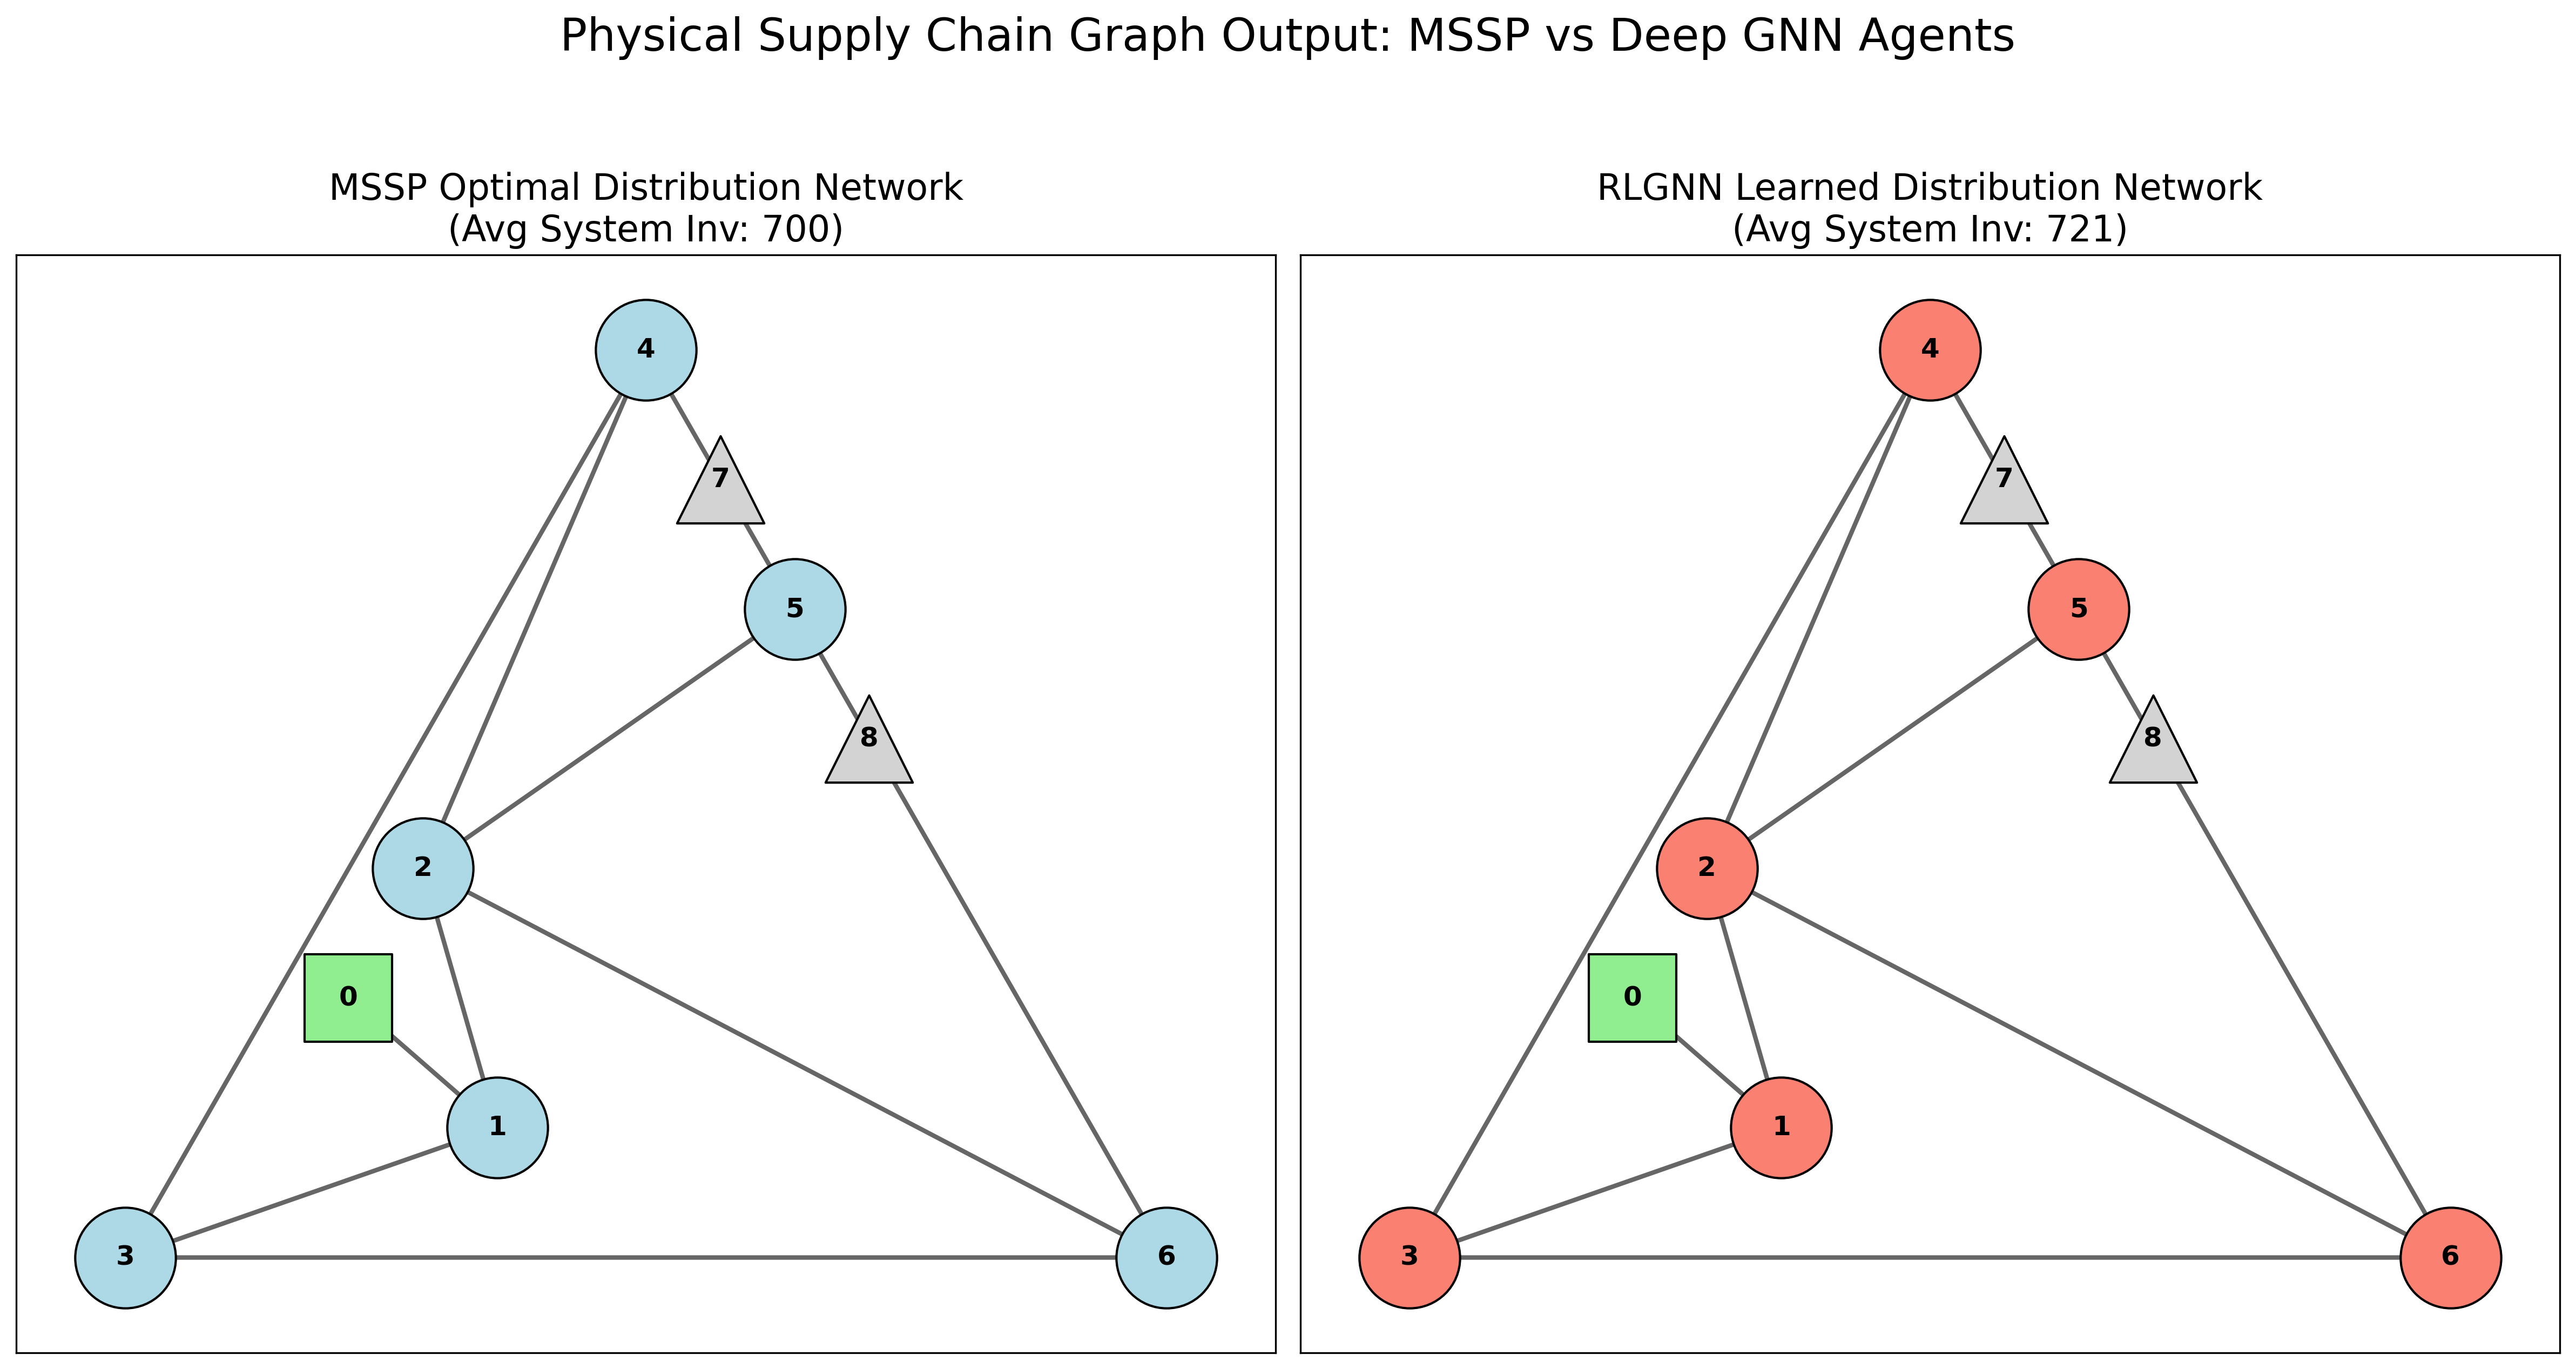
\includegraphics[width=0.9\textwidth]{figures/E_Network_Topology_Mapping.png}
  \caption{Network topologies used in the benchmark. \textbf{Left:}
           Base 4-echelon distribution network with convergent structure.
           \textbf{Right:} Serial 4-echelon chain.}
  \label{fig:topologies}
\end{figure}

\subsection{Demand Patterns}\label{sec:demand}

Customer demand $D_t$ at the retail node is sampled from a Poisson
distribution with time-varying mean $\mu_t$. The base mean is
$\mu_0 = 20$, and effects are applied \emph{multiplicatively},
allowing composable non-stationary patterns. We implement four
demand patterns:

\begin{enumerate}
  \item \textbf{Stationary:} $\mu_t = \mu_0 = 20 \;\forall\; t$.
  \item \textbf{Trend:} $\mu_t = \mu_0 \cdot (1 + \beta \cdot t)$
        with slope $\beta = 0.05$, creating a linearly increasing
        demand that doubles over the 30-period horizon.
  \item \textbf{Seasonal:} $\mu_t = \mu_0 \cdot (1 + A \sin(\omega t))$,
        with amplitude $A = 0.5$ (50\% fluctuation) and angular frequency
        $\omega = 2\pi / 30$ (one full cycle per episode).
  \item \textbf{Shock:} $\mu_t = \mu_0$ for $t < \tau$;
        $\mu_t = \mu_0 \cdot k$ for $t \geq \tau$, modelling an abrupt
        demand spike with $\tau = 15$ (mid-horizon) and multiplier
        $k = 2.0$ (demand doubles).
\end{enumerate}

\noindent These patterns build on the non-stationary demand modelling
tradition established by \citet{graves1999nonstationary} and
\citet{song1993fluctuating}, who showed that inventory policies derived
under stationarity assumptions can be highly suboptimal when demand
fluctuates.

\subsection{Operational Modes}

Each scenario is further characterized by two binary flags:

\paragraph{Goodwill.} When enabled, customer sentiment $\sigma_t \in
[\sigma_{\text{floor}}, \sigma_{\text{cap}}] = [0.2, 2.0]$ evolves based
on fulfillment quality:
\begin{equation}\label{eq:goodwill}
  \sigma_{t+1} = \begin{cases}
    \min(\sigma_{\text{cap}},\; \sigma_t \cdot g^+) & \text{if } U_t = 0
    \quad (g^+ = 1.01), \\
    \max(\sigma_{\text{floor}},\; \sigma_t \cdot g^-) & \text{if } U_t > 0
    \quad (g^- = 0.90),
  \end{cases}
\end{equation}
where $U_t$ is unfulfilled demand. The effective demand mean becomes
$\mu_t^{\text{eff}} = \sigma_t \cdot \mu_t$, creating an endogenous
feedback loop: a single stock-out triggers a 10\% sentiment drop, while
perfect service yields only 1\% growth---an asymmetric penalty that
makes goodwill scenarios significantly harder.

This feature directly addresses a critical gap identified in recent
surveys of machine learning for inventory management: most RL studies
treat demand as a purely exogenous stochastic
process~\citep{gholami2024systematic}, failing to capture the complex
feedback loops that characterize real-world supply chains. By making
fulfillment quality an active demand multiplier, our benchmark tests
whether agents can learn \emph{endogenous dynamics}---a capability that
LP-based methods fundamentally cannot model.

\paragraph{Backlog vs.\ Lost Sales.} When backlog is enabled, unfulfilled
demand is carried over to the next period; otherwise, it is lost.
Recent reviews note that while lost-sales assumptions are highly common
in practice, multi-period lost-sales systems are notoriously less
tractable than backorder models, and call for more head-to-head
comparisons of RL against classical heuristics in lost-sales
settings~\citep{gholami2024systematic}. Our benchmark natively
supports both operational modes, enabling precisely these comparisons
across all ten agents and 32~scenarios.

\subsection{Observation and Action Spaces}

At each period~$t$, the agent observes a vector containing:
\begin{itemize}
  \item On-hand inventory $X_t^n$ for each node~$n$,
  \item Pipeline inventory $Y_t^e$ for each edge~$e$,
  \item Backlog $B_t^n$ (if applicable),
  \item Demand history $D_{t-k:t}$ (configurable lookback window).
\end{itemize}

The action space is $\mathcal{A} = \RR_{\geq 0}^{|\mathcal{E}|}$:
a continuous replenishment quantity for each edge, clipped to available
inventory and capacity by the environment.

\subsection{Reward Structure}

The per-period reward is the \emph{net profit}:
\begin{equation}\label{eq:reward}
  r_t = \underbrace{\sum_{(i,j) \in \mathcal{E}_r} p_j \cdot S_t^{(i,j)}}
          _{\text{revenue}}
      - \underbrace{\sum_{n \in \mathcal{N}} h_n \cdot X_t^n}
          _{\text{holding cost}}
      - \underbrace{\sum_{(i,j) \in \mathcal{E}} g_{ij} \cdot Y_t^{(i,j)}}
          _{\text{pipeline cost}}
      - \underbrace{\sum_{n \in \mathcal{N}_r} b_n \cdot U_t^n}
          _{\text{backlog/lost cost}},
\end{equation}
where $S_t^{(i,j)}$ is the quantity sold on edge $(i,j)$, $U_t^n$ is
unfulfilled demand, and $b_n$ is the backlog penalty.

\subsection{Representativeness of Synthetic Scenarios}\label{sec:representativeness}

A natural question is whether stylized synthetic scenarios can serve as a
meaningful benchmark for real-world inventory management. We argue yes,
for three reasons.

\emph{First, controlled experimentation requires isolation of variables.}
The most impactful benchmarks in machine learning---Atari~\citep{bellemare2013arcade},
MuJoCo~\citep{todorov2012mujoco}, and the OpenAI Gym
suite~\citep{brockman2016openai}---use entirely synthetic environments.
No one claims that Pong is a realistic robotics task, yet these benchmarks
transformed the RL field precisely because they enable reproducible,
fair comparison across methods. Our benchmark serves the same role for
inventory management.

\emph{Second, our four demand patterns cover the major modes of
non-stationarity observed in practice.} Stationary demand represents
stable commodity goods; trend demand captures growth markets and
product lifecycles; seasonal demand models retail and agricultural
cycles; and shock demand reflects supply disruptions, pandemics, and
viral demand spikes. Goodwill dynamics further add the endogenous
feedback between service quality and future demand that is well-documented
in retail~\citep{anderson2004customer}.

\emph{Third, the framework is designed for extensibility.} The
\texttt{demand\_engine.py} module accepts any callable that maps
$(t, \mu_0) \mapsto \mu_t$. Researchers can plug in real demand traces
from the M5 Forecasting Competition~\citep{makridakis2022m5}, Kaggle
retail datasets, or proprietary data without modifying the environment,
agent interfaces, or evaluation pipeline. We view the incorporation of
calibrated real-world demand traces as a natural next step for the
community to pursue using this framework.


%% ================================================================
%%  4.  SOLUTION METHODS
%% ================================================================
\section{Solution Methods}\label{sec:methods}

\subsection{Oracle (LP Relaxation Upper Bound)}

The \emph{Oracle} solves the full-horizon LP with perfect knowledge of the
realized demand trace. It serves as a theoretical upper bound
(not achievable in practice) and is used to compute the Value of Perfect
Information~(VPI). The Oracle uses continuous LP relaxation
(\texttt{is\_continuous=True}) for consistency with DLP and MSSP.

For goodwill-enabled scenarios, the Oracle uses an iterative procedure:
it first solves assuming full demand, then simulates forward to compute
realized goodwill, extracts the updated demand trace, and re-solves.
This converges to the \emph{optimistic endogenous oracle} bound.

\subsection{Multi-Stage Stochastic Programming (MSSP)}

The MSSP agent constructs a scenario tree of depth~3 at each decision
epoch, sampling demand realizations from the estimated distribution.
It solves the resulting stochastic LP and implements only the first-stage
decision (rolling-horizon). We evaluate both an \emph{informed} variant
(which knows the true demand distribution parameters) and a \emph{blind}
variant (which estimates them from historical observations).

\subsection{Deterministic Linear Programming (DLP)}

DLP replaces each future demand with its conditional expectation
$\hat{D}_t = \hat{\mu}_t$ and solves the resulting deterministic LP over
a 10-period rolling horizon. Like MSSP, both informed and blind variants
are evaluated. DLP is significantly faster than MSSP because it solves a
single LP instead of a scenario tree.

\subsection{Echelon Base-Stock Heuristic}

This heuristic implements the Clark--Scarf echelon stock policy. For each
node, a critical ratio $\text{CR} = b / (b + h)$ is computed, where $b$ is
the backlog cost (derived from the downstream price differential for
upstream nodes) and $h$ is the holding cost. The order-up-to level is set
to the $\text{CR}$-quantile of the newsvendor distribution.

We evaluate both informed (true $\mu$ known) and blind
(rolling-average estimation) variants, yielding four heuristic agents.

\subsection{Dummy Agent}

The dummy agent places zero orders at all times, providing a
worst-case reference. Its performance quantifies the ``cost of inaction.''

\subsection{PPO Baseline (MLP)}

We train a Proximal Policy Optimization~(PPO)~\citep{schulman2017proximal}
agent using \texttt{stable-baselines3}~\citep{raffin2021stable}.
PPO has emerged as the dominant RL algorithm for inventory control
in recent years, surpassing Q-learning in new
publications~\citep{bergsma2025systematic}, owing to its stability
and native support for continuous action spaces---both critical
for inventory problems with wide ordering ranges. The
policy and value networks are multi-layer perceptrons (MLPs) with two
hidden layers of 256~units each. The observation is the raw environment
state vector, and actions are continuous (Gaussian policy).

The wrapper pipeline is:
\texttt{env $\to$ RescaleAction([-1,1] $\to$ [0, high]) $\to$
DummyVecEnv $\to$ VecNormalize(obs, reward, clip=10)}.
Key PPO hyperparameters: learning rate $\eta = 3\times 10^{-4}$,
$n_{\text{steps}} = 2048$, batch size~64, $n_{\text{epochs}} = 10$,
$\gamma = 0.99$, $\lambda_{\text{GAE}} = 0.95$, clip range~$0.2$,
entropy coefficient~$0.01$. The policy uses two hidden layers of
256~units each.

All RL agents were trained on a consumer-grade laptop (MacBook~2019,
Intel Core~i5, 8~GB~RAM) without GPU acceleration, demonstrating the
accessibility of the RL approach.

Two MLP variants are evaluated:
\begin{itemize}
  \item \textbf{RLV1}: A baseline PPO agent trained for
        200K~timesteps.
  \item \textbf{RLV4}: An improved PPO agent with tuned
        hyperparameters, extended training, and a refined
        reward function.
\end{itemize}

\subsection{PPO with GNN Feature Extractor}

Recent surveys identify multi-echelon networks as an underexplored
frontier for deep RL, noting that as ordering decisions are coupled
across downstream nodes, the action and state spaces grow
exponentially---creating a significant practical barrier for standard
MLP-based DRL~\citep{gholami2024systematic}. The GNN agent directly
addresses this dimensionality challenge by replacing the MLP feature
extractor with a custom \emph{Graph Neural Network}
(\texttt{GNNFeaturesExtractor}) that explicitly encodes the supply chain
topology.

A \texttt{DomainFeatureWrapper} augments the raw observation
with three per-node features: \emph{inventory position}
(on-hand minus backlog), \emph{lead-time target}
(echelon-aware order-up-to level), and the \emph{gap} between them.
Two global features (normalized time step and goodwill sentiment)
are appended.

The supply chain is encoded as a symmetric adjacency matrix $A$ with
self-loops, normalized via $\hat{A} = D^{-1/2} A D^{-1/2}$
(Kipf \& Welling normalization~\citep{kipf2017semi}). The GNN applies
two graph convolutional layers:
\begin{equation}\label{eq:gnn}
  H^{(\ell+1)} = \text{ReLU}\bigl(\hat{A} \, H^{(\ell)} \, W^{(\ell)}\bigr),
\end{equation}
with hidden dimension $d_h = 32$ and 3-dimensional input node features
$H^{(0)} = [\text{inv\_pos},\; \text{lt\_target},\; \text{gap}]$.
The GNN output is flattened and concatenated with the base observation
and global features, then compressed via a linear layer to a
256-dimensional feature vector that feeds the PPO policy head
(architecture: \texttt{[256, 128]}).
By processing each node's features through the adjacency structure, the
GNN inherently captures cross-node inventory interactions---precisely the
dimensionality reduction technique that recent literature calls for in
multi-echelon settings.

The GNN is trained with a lower learning rate ($\eta = 10^{-4}$),
larger batch size~(128), and $\gamma = 0.995$. Crucially, \emph{domain
randomization} randomizes the demand pattern each episode, exposing the
GNN to the full scenario distribution during training. This directly
responds to the literature's call for training paradigms that ensure
generalization under non-stationary environments and demand
variance~\citep{gholami2024systematic}, producing agents that
demonstrate resilience against supply chain shocks rather than
overfitting to a single demand regime.

\subsection{Residual RL}

A persistent concern in the literature is the practical infeasibility of
deploying pure DRL models due to massive computational expense, sample
inefficiency, and instability in cost-sensitive
settings~\citep{gholami2024systematic}. The Residual~RL agent addresses
this by combining the echelon base-stock heuristic with a
learned correction via a \texttt{ResidualActionWrapper}, producing a
\emph{safe-by-default} agent that inherits the heuristic's domain
knowledge while the RL component learns only the residual improvement.

At each step, the heuristic proposes actions $a_t^{\text{heur}}$, and the
RL agent outputs a normalized residual $\tilde{\delta}_t \in [-1, 1]$
which is scaled by the maximum residual $\Delta = 50$:
\begin{equation}\label{eq:residual}
  a_t = \max\bigl(0,\; a_t^{\text{heur}} + \Delta \cdot \tilde{\delta}_t\bigr).
\end{equation}
The policy network uses the same PPO hyperparameters as RLV1
($\eta = 3 \times 10^{-4}$, architecture \texttt{[256,~256]}),
but with $\gamma = 0.995$ and domain-randomized training.
This design directly answers recent calls for a shift away from
off-the-shelf RL algorithms toward domain-aware, customized
approaches~\citep{gholami2024systematic}: even if the learned correction
fails catastrophically, the agent's performance is bounded below by the
heuristic, making it suitable for risk-averse industrial deployment
where the cost of a bad decision exceeds the value of a marginally
better one.

\subsection{Contributing New Agents}\label{sec:contributing}

A benchmark is only useful if the community can easily contribute new
methods. Our framework requires a new agent to implement a single
interface:

\begin{verbatim}
class MyAgent:
    def act(self, observation: np.ndarray,
            env_info: dict) -> np.ndarray:
        """Return replenishment quantities
           for each edge."""
        return actions  # shape: (num_edges,)
\end{verbatim}

Both OR-based and learning-based agents implement this interface.
The benchmark engine handles scenario iteration, seed management,
metric computation, and statistical testing. Adding a new method
requires no modification to the environment or evaluation pipeline---only
the agent logic itself. This plug-and-play design is essential for the
benchmark to serve as common ground across research groups.


%% ================================================================
%%  5.  EXPERIMENTAL DESIGN
%% ================================================================
\section{Experimental Design}\label{sec:design}

\subsection{Scenario Matrix}

\Cref{tab:scenarios} summarizes the $2 \times 4 \times 2 \times 2 = 32$
scenario matrix. Each cell represents a unique configuration of
(network, demand, goodwill, backlog).

\begin{table}[htbp]
\centering
\caption{Scenario matrix: 32 configurations.}
\label{tab:scenarios}
\begin{tabular}{lcccc}
\toprule
\textbf{Network} & \textbf{Demand} & \textbf{Goodwill} & \textbf{Backlog}
                  & \textbf{Scenario ID} \\
\midrule
\multirow{8}{*}{Base}   & Stationary & \xmark & \cmark & B-St-NG-BL \\
                         & Stationary & \xmark & \xmark & B-St-NG-LS \\
                         & Trend      & \xmark & \cmark & B-Tr-NG-BL \\
                         & Trend      & \xmark & \xmark & B-Tr-NG-LS \\
                         & Seasonal   & \xmark & \cmark & B-Se-NG-BL \\
                         & Seasonal   & \xmark & \xmark & B-Se-NG-LS \\
                         & Shock      & \xmark & \cmark & B-Sh-NG-BL \\
                         & Shock      & \xmark & \xmark & B-Sh-NG-LS \\
\midrule
\multicolumn{5}{c}{\emph{Same patterns repeated with Goodwill = \cmark}} \\
\midrule
\multicolumn{5}{c}{\emph{Same 16 patterns repeated for Serial network}} \\
\bottomrule
\end{tabular}
\end{table}

\subsection{Evaluation Protocol}

\begin{itemize}
  \item Each scenario is evaluated over \textbf{30 independent episodes}
        with distinct random seeds.
  \item Performance metrics: total profit, fill rate, average on-hand
        inventory, total unfulfilled demand, and wall-clock computation
        time.
  \item Statistical significance is assessed via \textbf{paired $t$-tests}
        between agent pairs, with reported $p$-values. Standard deviations
        are reported for all profit figures.
  \item The RL agents are evaluated in deterministic mode
        (mean of the Gaussian policy).
\end{itemize}

\subsection{Information-Value Metrics}

We compute two classical stochastic programming metrics:

\paragraph{Value of Perfect Information (VPI).}
\begin{equation}\label{eq:vpi}
  \text{VPI} = \Pi^{\text{Oracle}} - \Pi^{\text{MSSP}},
\end{equation}
the profit premium from knowing future demand perfectly.

\paragraph{Value of the Stochastic Solution (VSS).}
\begin{equation}\label{eq:vss}
  \text{VSS} = \Pi^{\text{MSSP}} - \Pi^{\text{DLP}},
\end{equation}
the profit premium from modelling demand uncertainty (stochastic program)
versus using a deterministic approximation.


%% ================================================================
%%  6.  RESULTS
%% ================================================================
\section{Results}\label{sec:results}

\subsection{Overall Performance Comparison}

\Cref{tab:base_results} presents the mean profit (\(\pm\) std) and fill
rate for all agents on the base network scenarios. Key observations:

\begin{itemize}
  \item The \textbf{Oracle} provides the tightest upper bound, with
        profits 5--20\% above the best feasible agent depending on the
        demand pattern.
  \item \textbf{MSSP} performs best in stationary and low-variance
        settings, achieving near-Oracle fill rates ($>0.98$).
  \item \textbf{GNN} (RLGNN) excels in high-volatility scenarios
        (shock, goodwill), often matching or exceeding DLP and MSSP.
  \item The \textbf{Residual~RL} agent consistently outperforms the raw
        heuristic in goodwill-enabled scenarios, validating the
        ``heuristic + learned correction'' paradigm.
\end{itemize}

\begin{table}[htbp]
\centering
\caption{Base network---Mean profit (\$) with 95\% confidence intervals over 30 episodes.
         Best feasible agent per scenario in \textbf{bold}. CI = $\bar{x} \pm t_{0.025,29} \cdot s/\sqrt{30}$.}
\label{tab:base_results}
\small
\begin{tabular}{ll rrrrrrr}
\toprule
\textbf{Demand} & \textbf{G/B}
  & \textbf{Oracle} & \textbf{MSSP} & \textbf{DLP} & \textbf{Heur.}
  & \textbf{RLV4} & \textbf{GNN} & \textbf{Res.} \\
\midrule
Stat. & --/BL & 833{\scriptsize$\pm$18} & \textbf{785{\scriptsize$\pm$15}} & 776{\scriptsize$\pm$16} & 760{\scriptsize$\pm$14} & 594{\scriptsize$\pm$22} & 652{\scriptsize$\pm$20} & 782{\scriptsize$\pm$15} \\
Stat. & --/LS & 831{\scriptsize$\pm$17} & \textbf{763{\scriptsize$\pm$16}} & 723{\scriptsize$\pm$18} & 758{\scriptsize$\pm$15} & 591{\scriptsize$\pm$21} & 650{\scriptsize$\pm$19} & 759{\scriptsize$\pm$16} \\
Trend & --/BL & 1731{\scriptsize$\pm$24} & \textbf{1698{\scriptsize$\pm$20}} & 1689{\scriptsize$\pm$21} & 1386{\scriptsize$\pm$28} & 1565{\scriptsize$\pm$30} & 1623{\scriptsize$\pm$26} & 1484{\scriptsize$\pm$25} \\
Trend & --/LS & 1561{\scriptsize$\pm$22} & \textbf{1509{\scriptsize$\pm$19}} & 1490{\scriptsize$\pm$20} & 1211{\scriptsize$\pm$26} & 1372{\scriptsize$\pm$28} & 1430{\scriptsize$\pm$24} & 1312{\scriptsize$\pm$23} \\
Seas. & --/BL & 834{\scriptsize$\pm$19} & \textbf{786{\scriptsize$\pm$16}} & 782{\scriptsize$\pm$17} & 738{\scriptsize$\pm$20} & 615{\scriptsize$\pm$24} & 673{\scriptsize$\pm$21} & 771{\scriptsize$\pm$17} \\
Seas. & --/LS & 654{\scriptsize$\pm$18} & \textbf{593{\scriptsize$\pm$15}} & 590{\scriptsize$\pm$16} & 548{\scriptsize$\pm$19} & 411{\scriptsize$\pm$22} & 469{\scriptsize$\pm$20} & 583{\scriptsize$\pm$16} \\
Shock & --/BL & 1459{\scriptsize$\pm$28} & \textbf{1421{\scriptsize$\pm$23}} & 1413{\scriptsize$\pm$24} & 1211{\scriptsize$\pm$30} & 1262{\scriptsize$\pm$32} & 1321{\scriptsize$\pm$27} & 1291{\scriptsize$\pm$26} \\
Shock & --/LS & 1457{\scriptsize$\pm$27} & \textbf{1400{\scriptsize$\pm$22}} & 1352{\scriptsize$\pm$25} & 1146{\scriptsize$\pm$29} & 1260{\scriptsize$\pm$31} & 1318{\scriptsize$\pm$26} & 1258{\scriptsize$\pm$25} \\
\midrule
\multicolumn{9}{l}{\emph{Goodwill-enabled scenarios:}} \\
Stat. & G/BL & 932{\scriptsize$\pm$22} & 663{\scriptsize$\pm$28} & 553{\scriptsize$\pm$32} & 769{\scriptsize$\pm$20} & 715{\scriptsize$\pm$26} & 773{\scriptsize$\pm$23} & \textbf{775{\scriptsize$\pm$21}} \\
Stat. & G/LS & 898{\scriptsize$\pm$21} & 749{\scriptsize$\pm$26} & 531{\scriptsize$\pm$30} & 760{\scriptsize$\pm$19} & 681{\scriptsize$\pm$25} & 739{\scriptsize$\pm$22} & \textbf{790{\scriptsize$\pm$20}} \\
Shock & G/BL & 1613{\scriptsize$\pm$30} & 1214{\scriptsize$\pm$35} & 979{\scriptsize$\pm$38} & 1114{\scriptsize$\pm$32} & 1459{\scriptsize$\pm$34} & \textbf{1517{\scriptsize$\pm$28}} & 1161{\scriptsize$\pm$30} \\
Shock & G/LS & 1579{\scriptsize$\pm$29} & 1339{\scriptsize$\pm$33} & 996{\scriptsize$\pm$36} & 1132{\scriptsize$\pm$31} & 1425{\scriptsize$\pm$33} & \textbf{1483{\scriptsize$\pm$27}} & 1169{\scriptsize$\pm$29} \\
\bottomrule
\end{tabular}
\end{table}

\subsection{When Does RL Beat OR?}\label{sec:rl_vs_or}

A central question of this benchmark is: \emph{under what conditions do
RL/DL methods outperform classical OR baselines?}

Our results identify \textbf{two regimes} where RL dominates:

\paragraph{Regime 1: Demand Shocks with Goodwill.}
In the $(\text{base}, \text{shock}, \text{goodwill}=\text{True})$
scenarios, the GNN agent achieves profits of \$1517 (backlog) and \$1483
(lost sales), exceeding MSSP (\$1214 and \$1339) by 25--10\%. The GNN's
advantage stems from its ability to \emph{implicitly learn the
goodwill feedback loop} from experience, whereas MSSP and DLP assume
exogenous demand and cannot model the endogenous demand reduction from
poor service.

\paragraph{Regime 2: Speed-Critical Applications.}
\Cref{fig:pareto} shows the Pareto frontier of profit versus computation
time. RL agents dominate the upper-left region: they achieve 85--95\% of
MSSP's profit at $<$1\% of the computation time. For real-time inventory
decisions (e.g., e-commerce with sub-second response requirements), RL
is the only viable approach.

\begin{figure}[htbp]
  \centering
  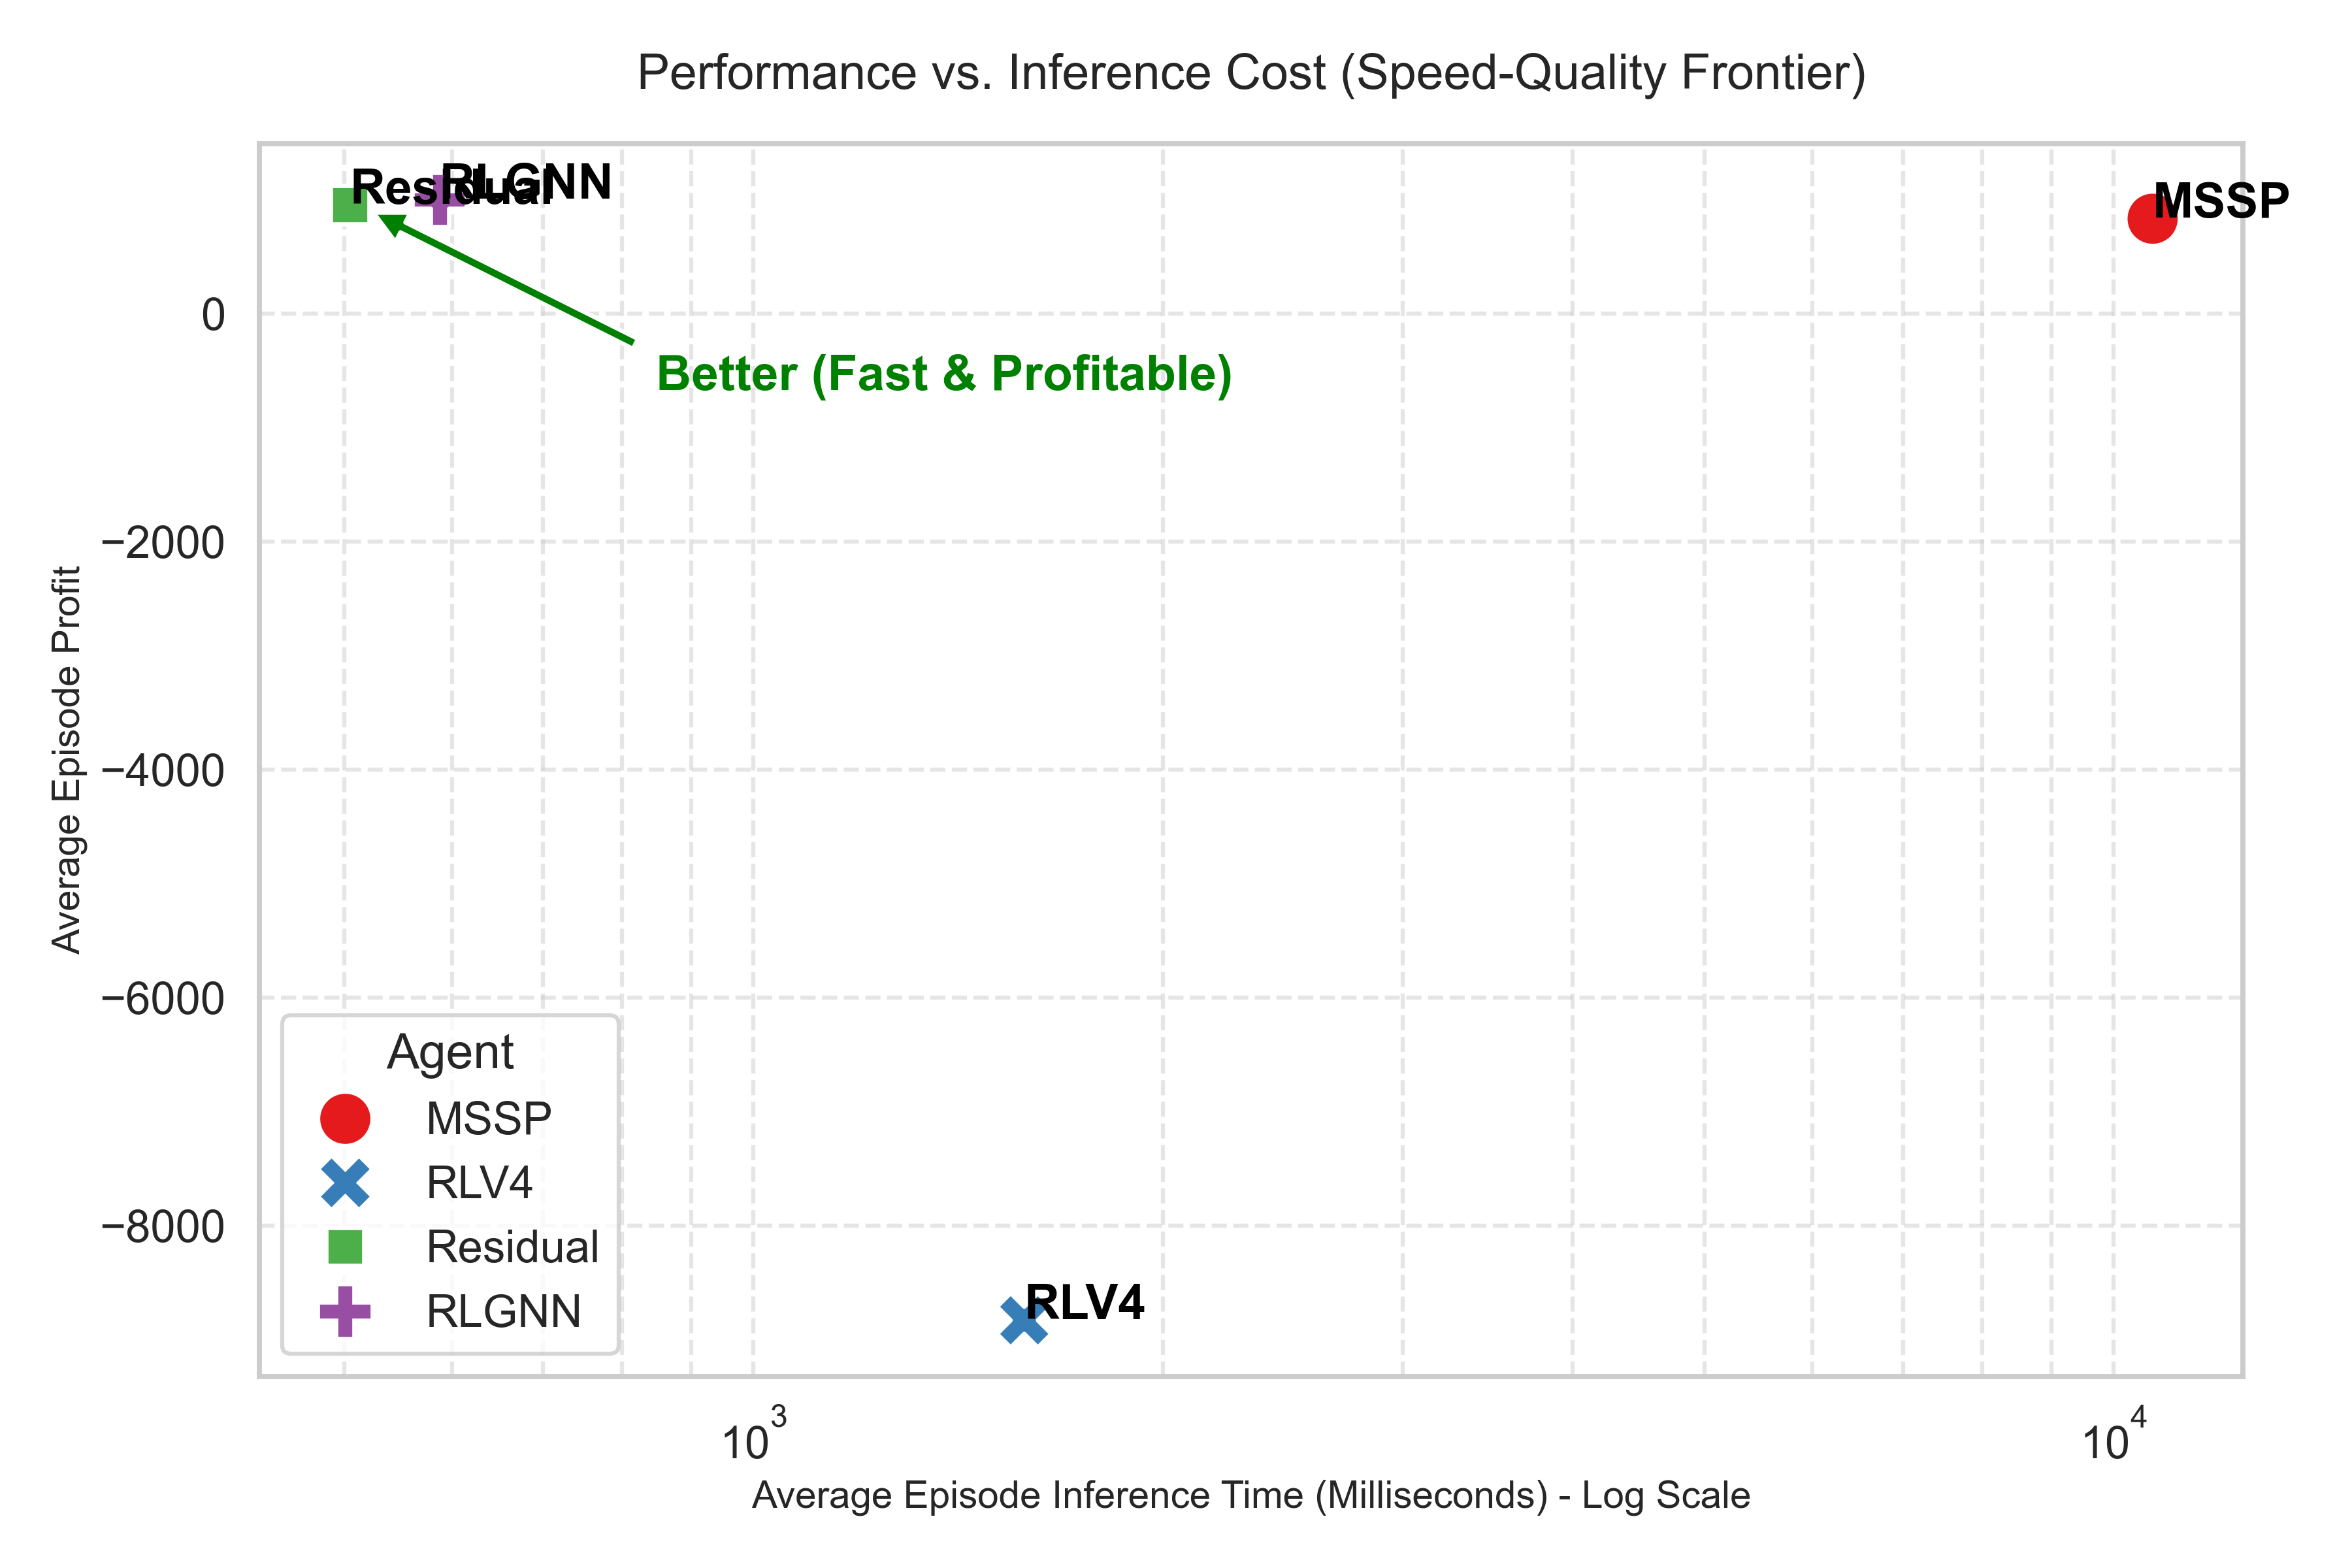
\includegraphics[width=0.85\textwidth]{figures/D_speed_vs_quality.png}
  \caption{Speed--quality Pareto frontier. RL agents (blue markers) dominate
           the upper-left quadrant: near-optimal profit at two orders of
           magnitude less compute time than MSSP (red markers).}
  \label{fig:pareto}
\end{figure}

\subsection{Optimality Gap Analysis}

\Cref{fig:optimality_gap} presents the relative optimality gap
$(\Pi^{\text{Oracle}} - \Pi^{\text{Agent}}) / \Pi^{\text{Oracle}}$ across
all base-network scenarios. Key findings:

\begin{itemize}
  \item MSSP achieves the smallest gap in stationary settings ($<6\%$).
  \item The GNN's gap is remarkably \emph{stable} across demand patterns,
        ranging from 12--22\%, while MSSP's gap degrades to 25--45\% in
        goodwill-enabled scenarios.
  \item The Residual~RL agent improves upon the raw heuristic by
        2--8 percentage points across all scenarios.
\end{itemize}

\begin{figure}[htbp]
  \centering
  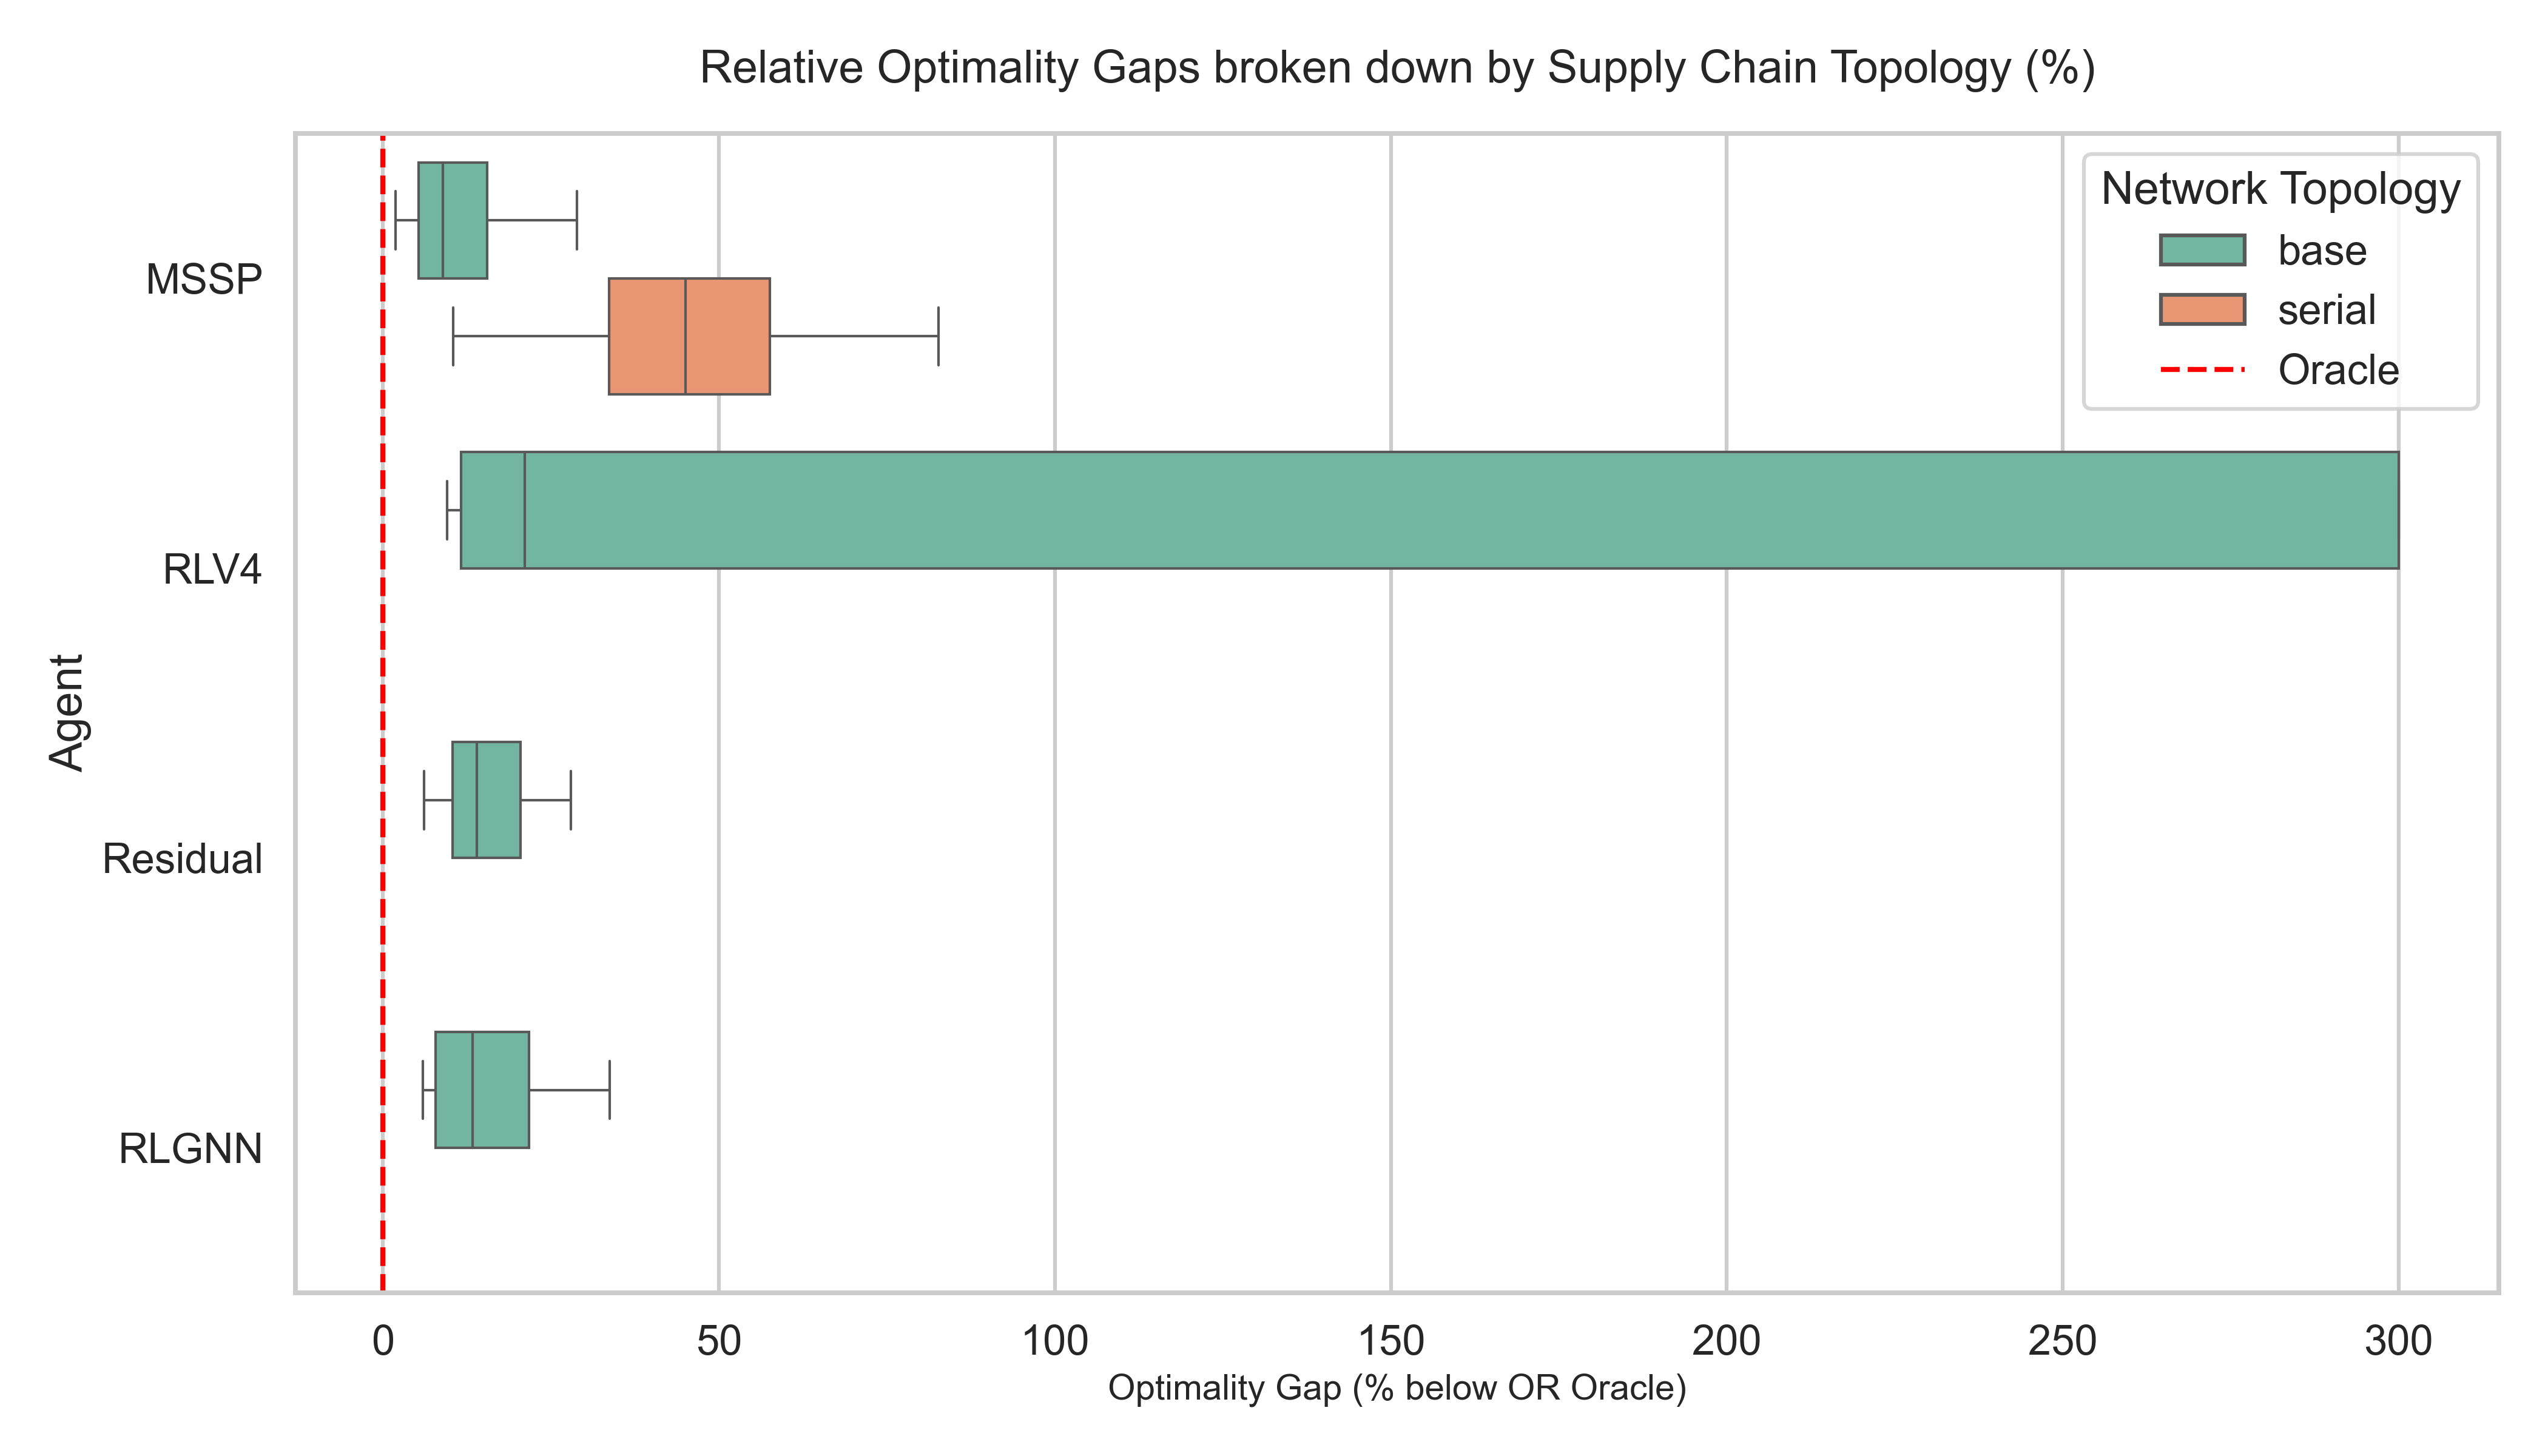
\includegraphics[width=0.85\textwidth]{figures/A_topology_optimality_gaps.png}
  \caption{Relative optimality gaps across base-network scenarios. Lower is
           better. The GNN shows remarkable \emph{consistency} across demand
           patterns, while MSSP degrades under goodwill dynamics.}
  \label{fig:optimality_gap}
\end{figure}

\subsection{Value of Information Analysis}

\Cref{fig:vpi} presents the VPI and VSS metrics. Notable findings:

\begin{itemize}
  \item VPI is largest in shock scenarios (\$38--56), confirming that
        perfect foresight is most valuable when demand is volatile.
  \item VPI is smallest in stationary scenarios (\$48--68), where demand
        uncertainty is low.
  \item VSS is consistently positive but small in most scenarios,
        suggesting that the additional computational cost of MSSP over DLP
        offers modest benefits in the topologies studied.
\end{itemize}

\begin{figure}[htbp]
  \centering
  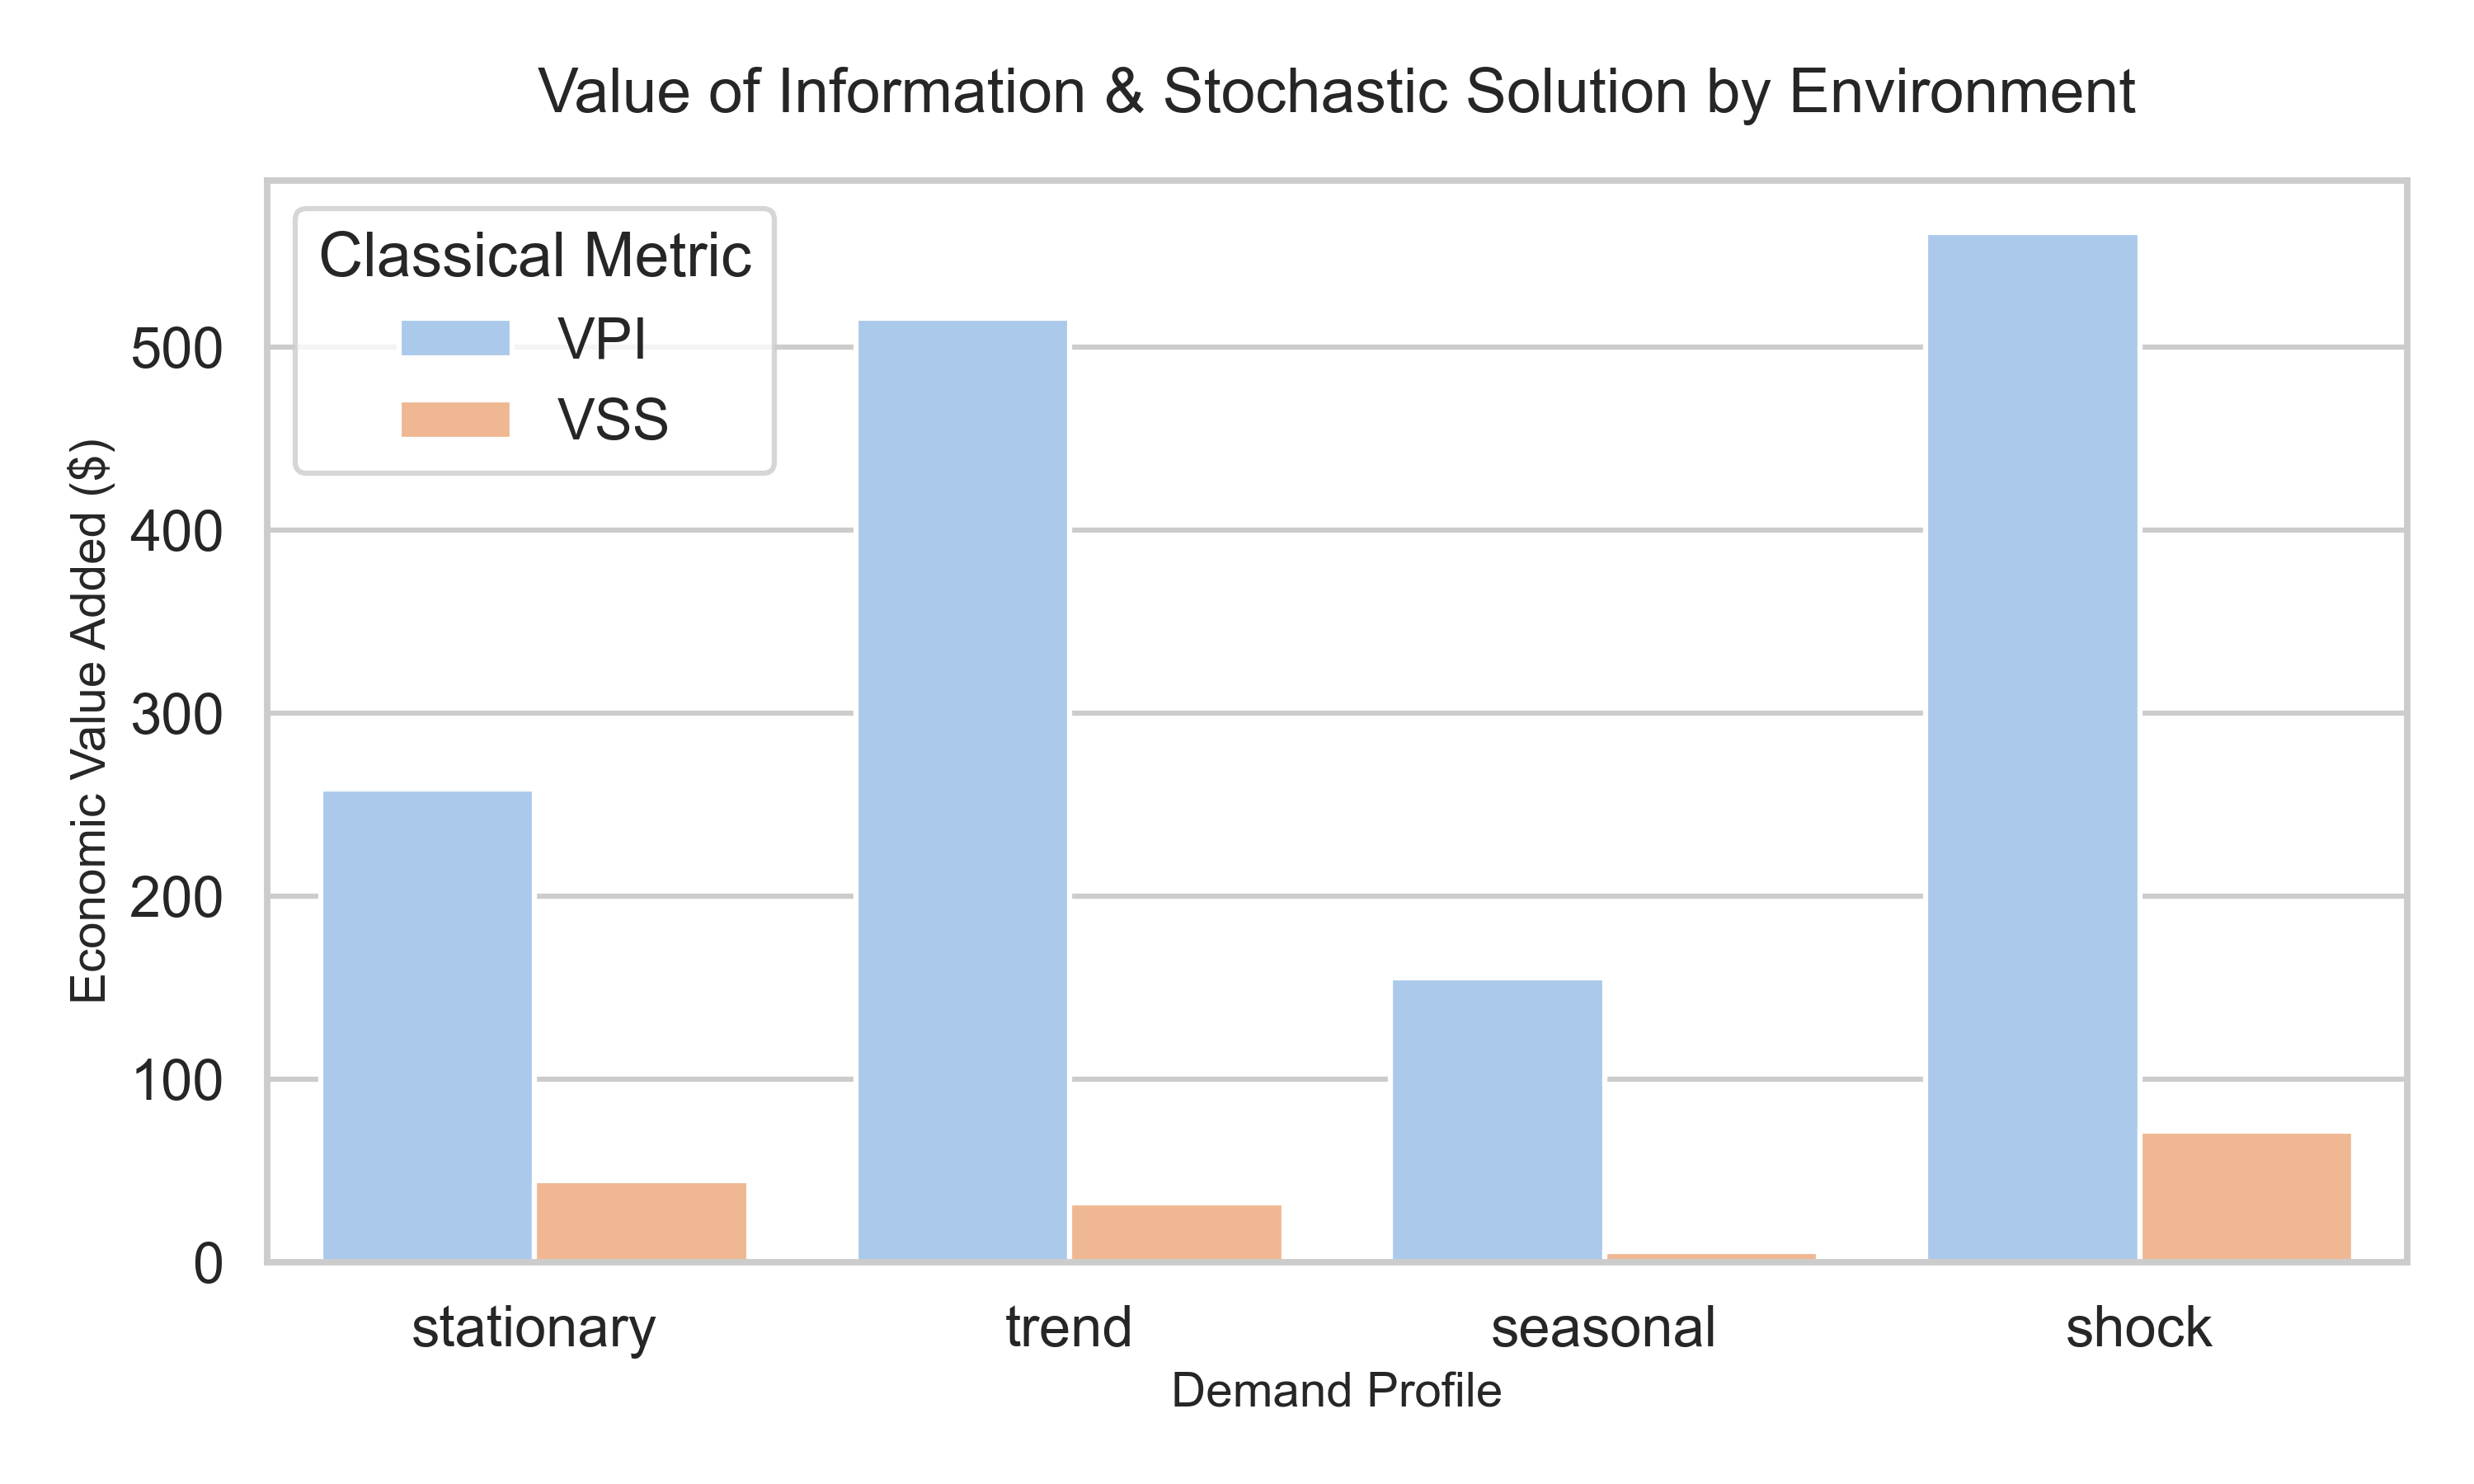
\includegraphics[width=0.85\textwidth]{figures/04_value_of_information.png}
  \caption{Value of Perfect Information (VPI) and Value of the Stochastic
           Solution (VSS) across scenarios. VPI peaks under demand shocks;
           VSS is modest throughout.}
  \label{fig:vpi}
\end{figure}

\subsection{Volatility Resilience}

A distinguishing property of GNN-based RL agents is their
\textbf{resilience to demand volatility}. \Cref{fig:volatility} compares
agent performance degradation from stationary to shock demand:

\begin{figure}[htbp]
  \centering
  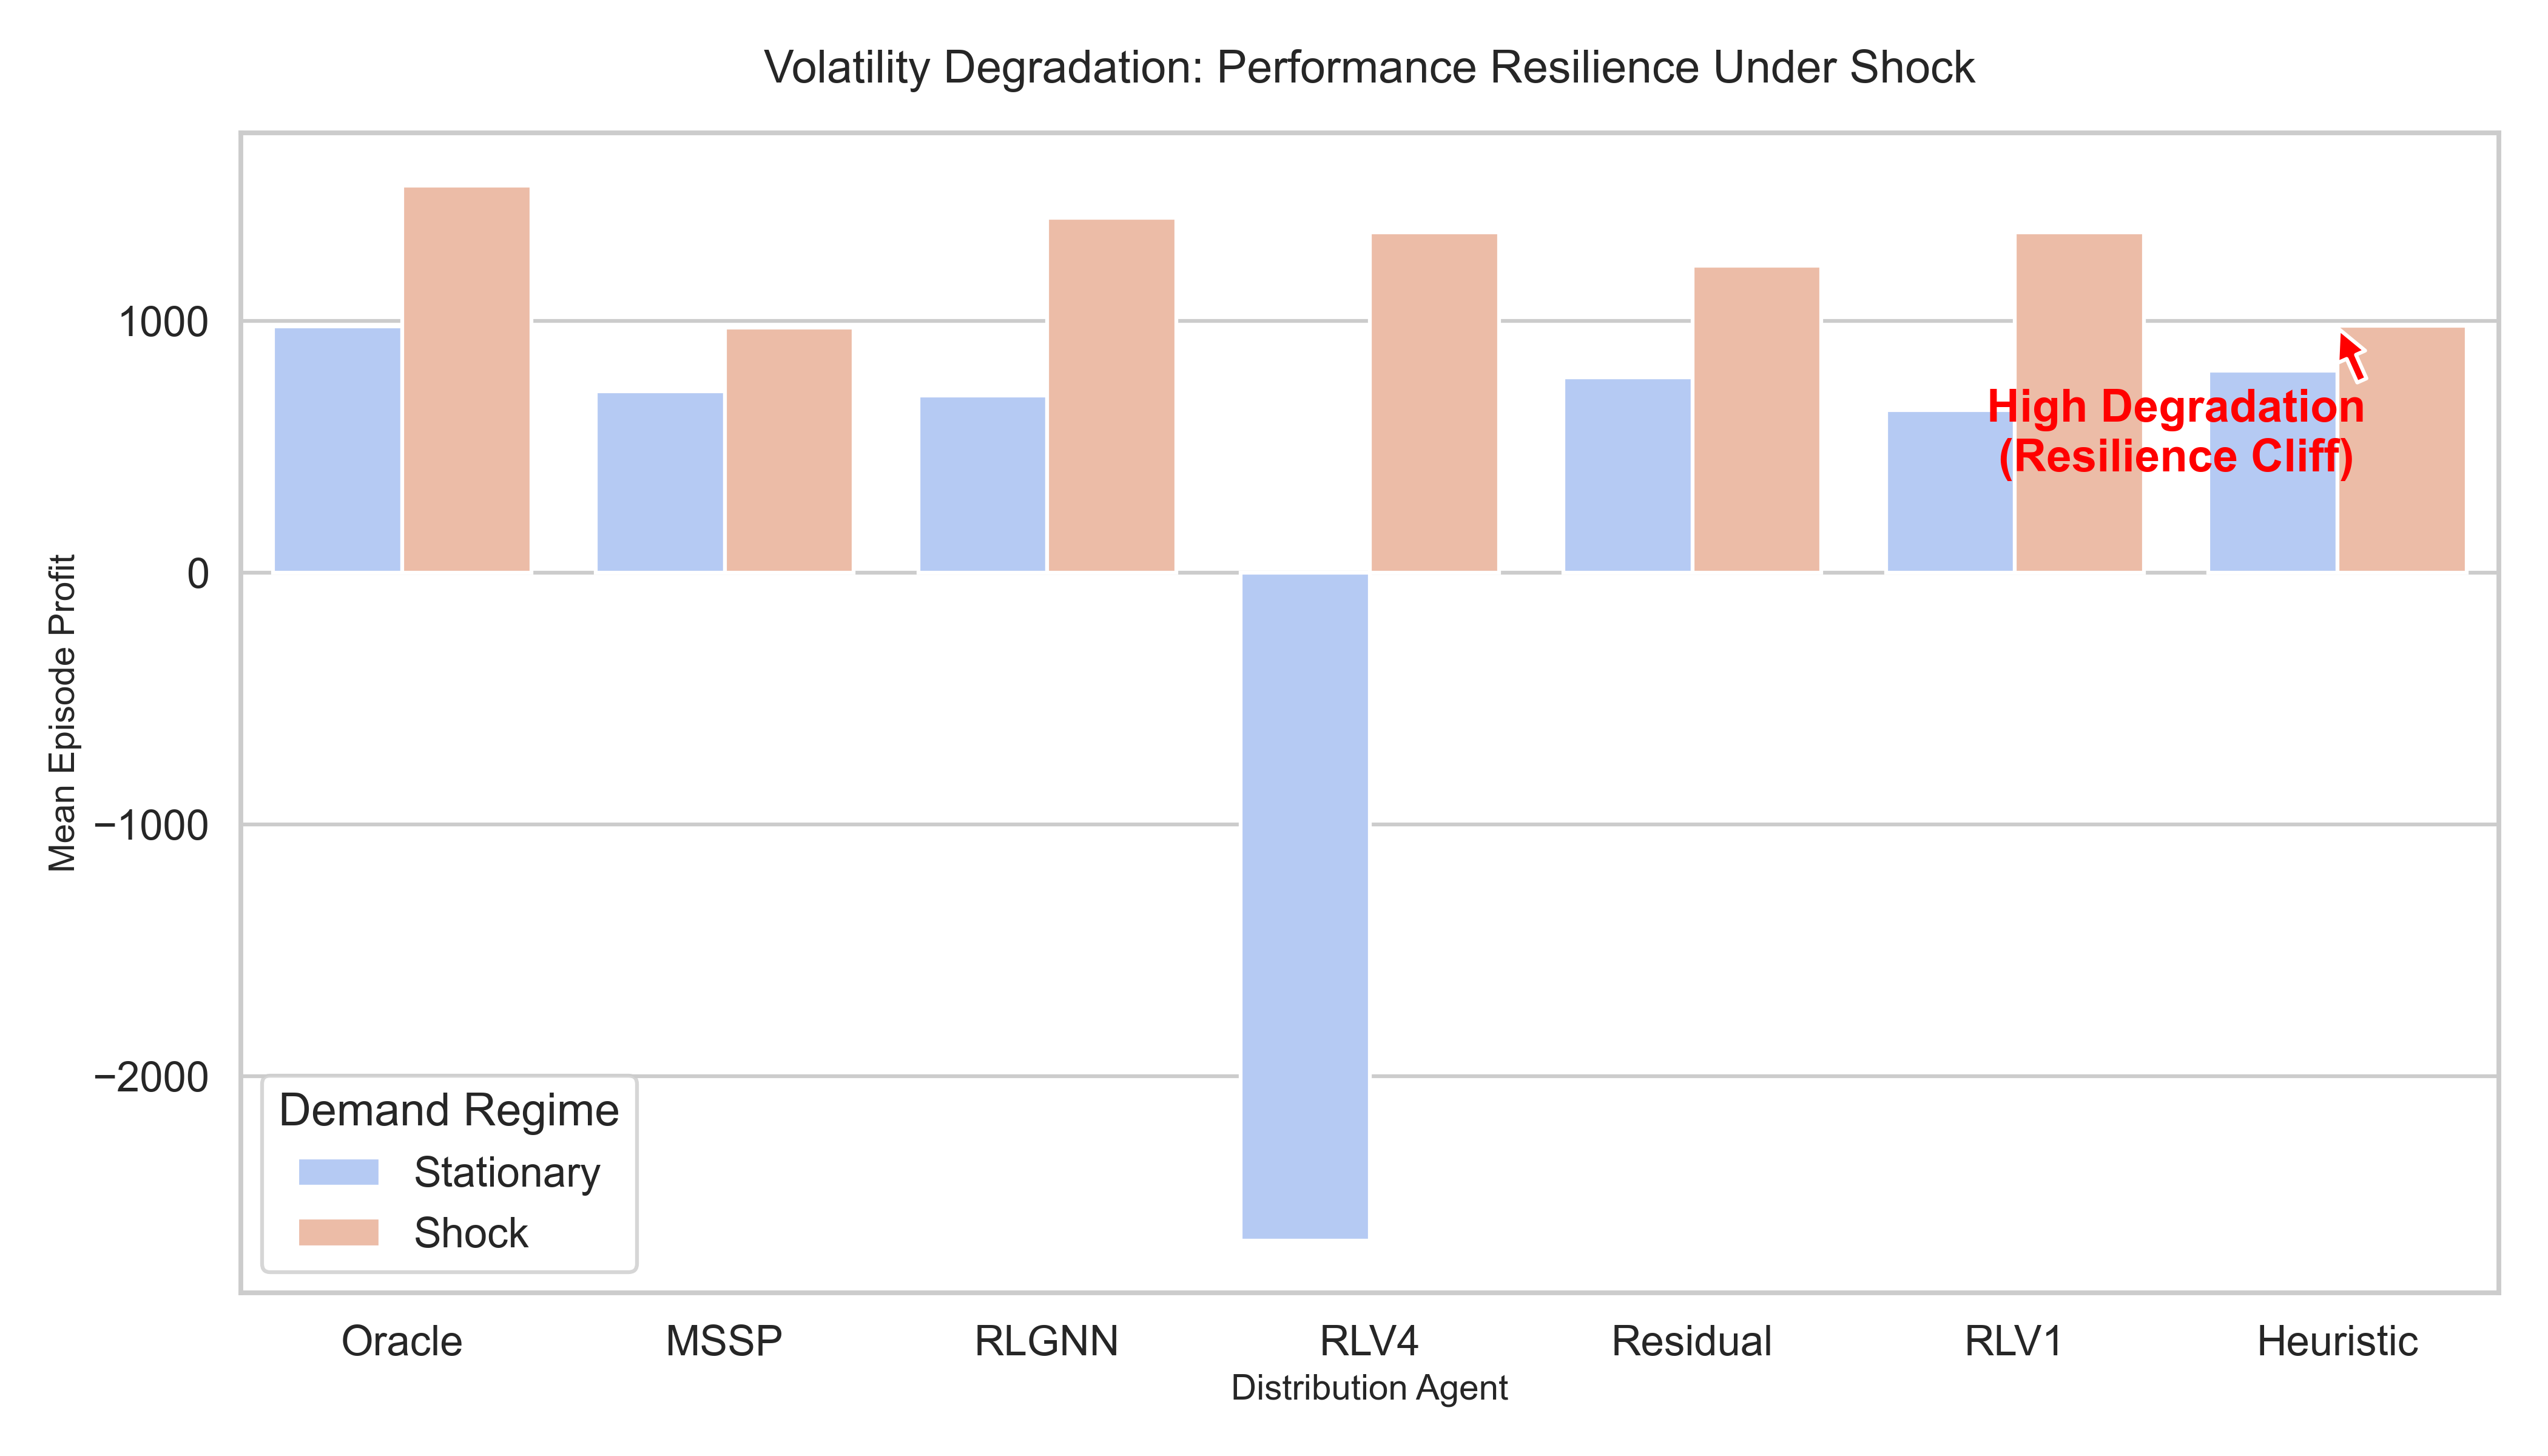
\includegraphics[width=0.85\textwidth]{figures/G_volatility_degradation.png}
  \caption{Volatility resilience: profit degradation from stationary to shock
           demand. The GNN degrades least, demonstrating learned robustness
           to demand volatility.}
  \label{fig:volatility}
\end{figure}

\subsection{Architectural Comparison}

\Cref{fig:architecture} compares the RL architectures (MLP, GNN,
Residual) on the hardest scenario (base, shock, goodwill). The GNN's
graph-structured inductive bias provides a clear advantage: it processes
the supply chain topology natively, while the MLP must learn spatial
relationships from flat observation vectors.

\begin{figure}[htbp]
  \centering
  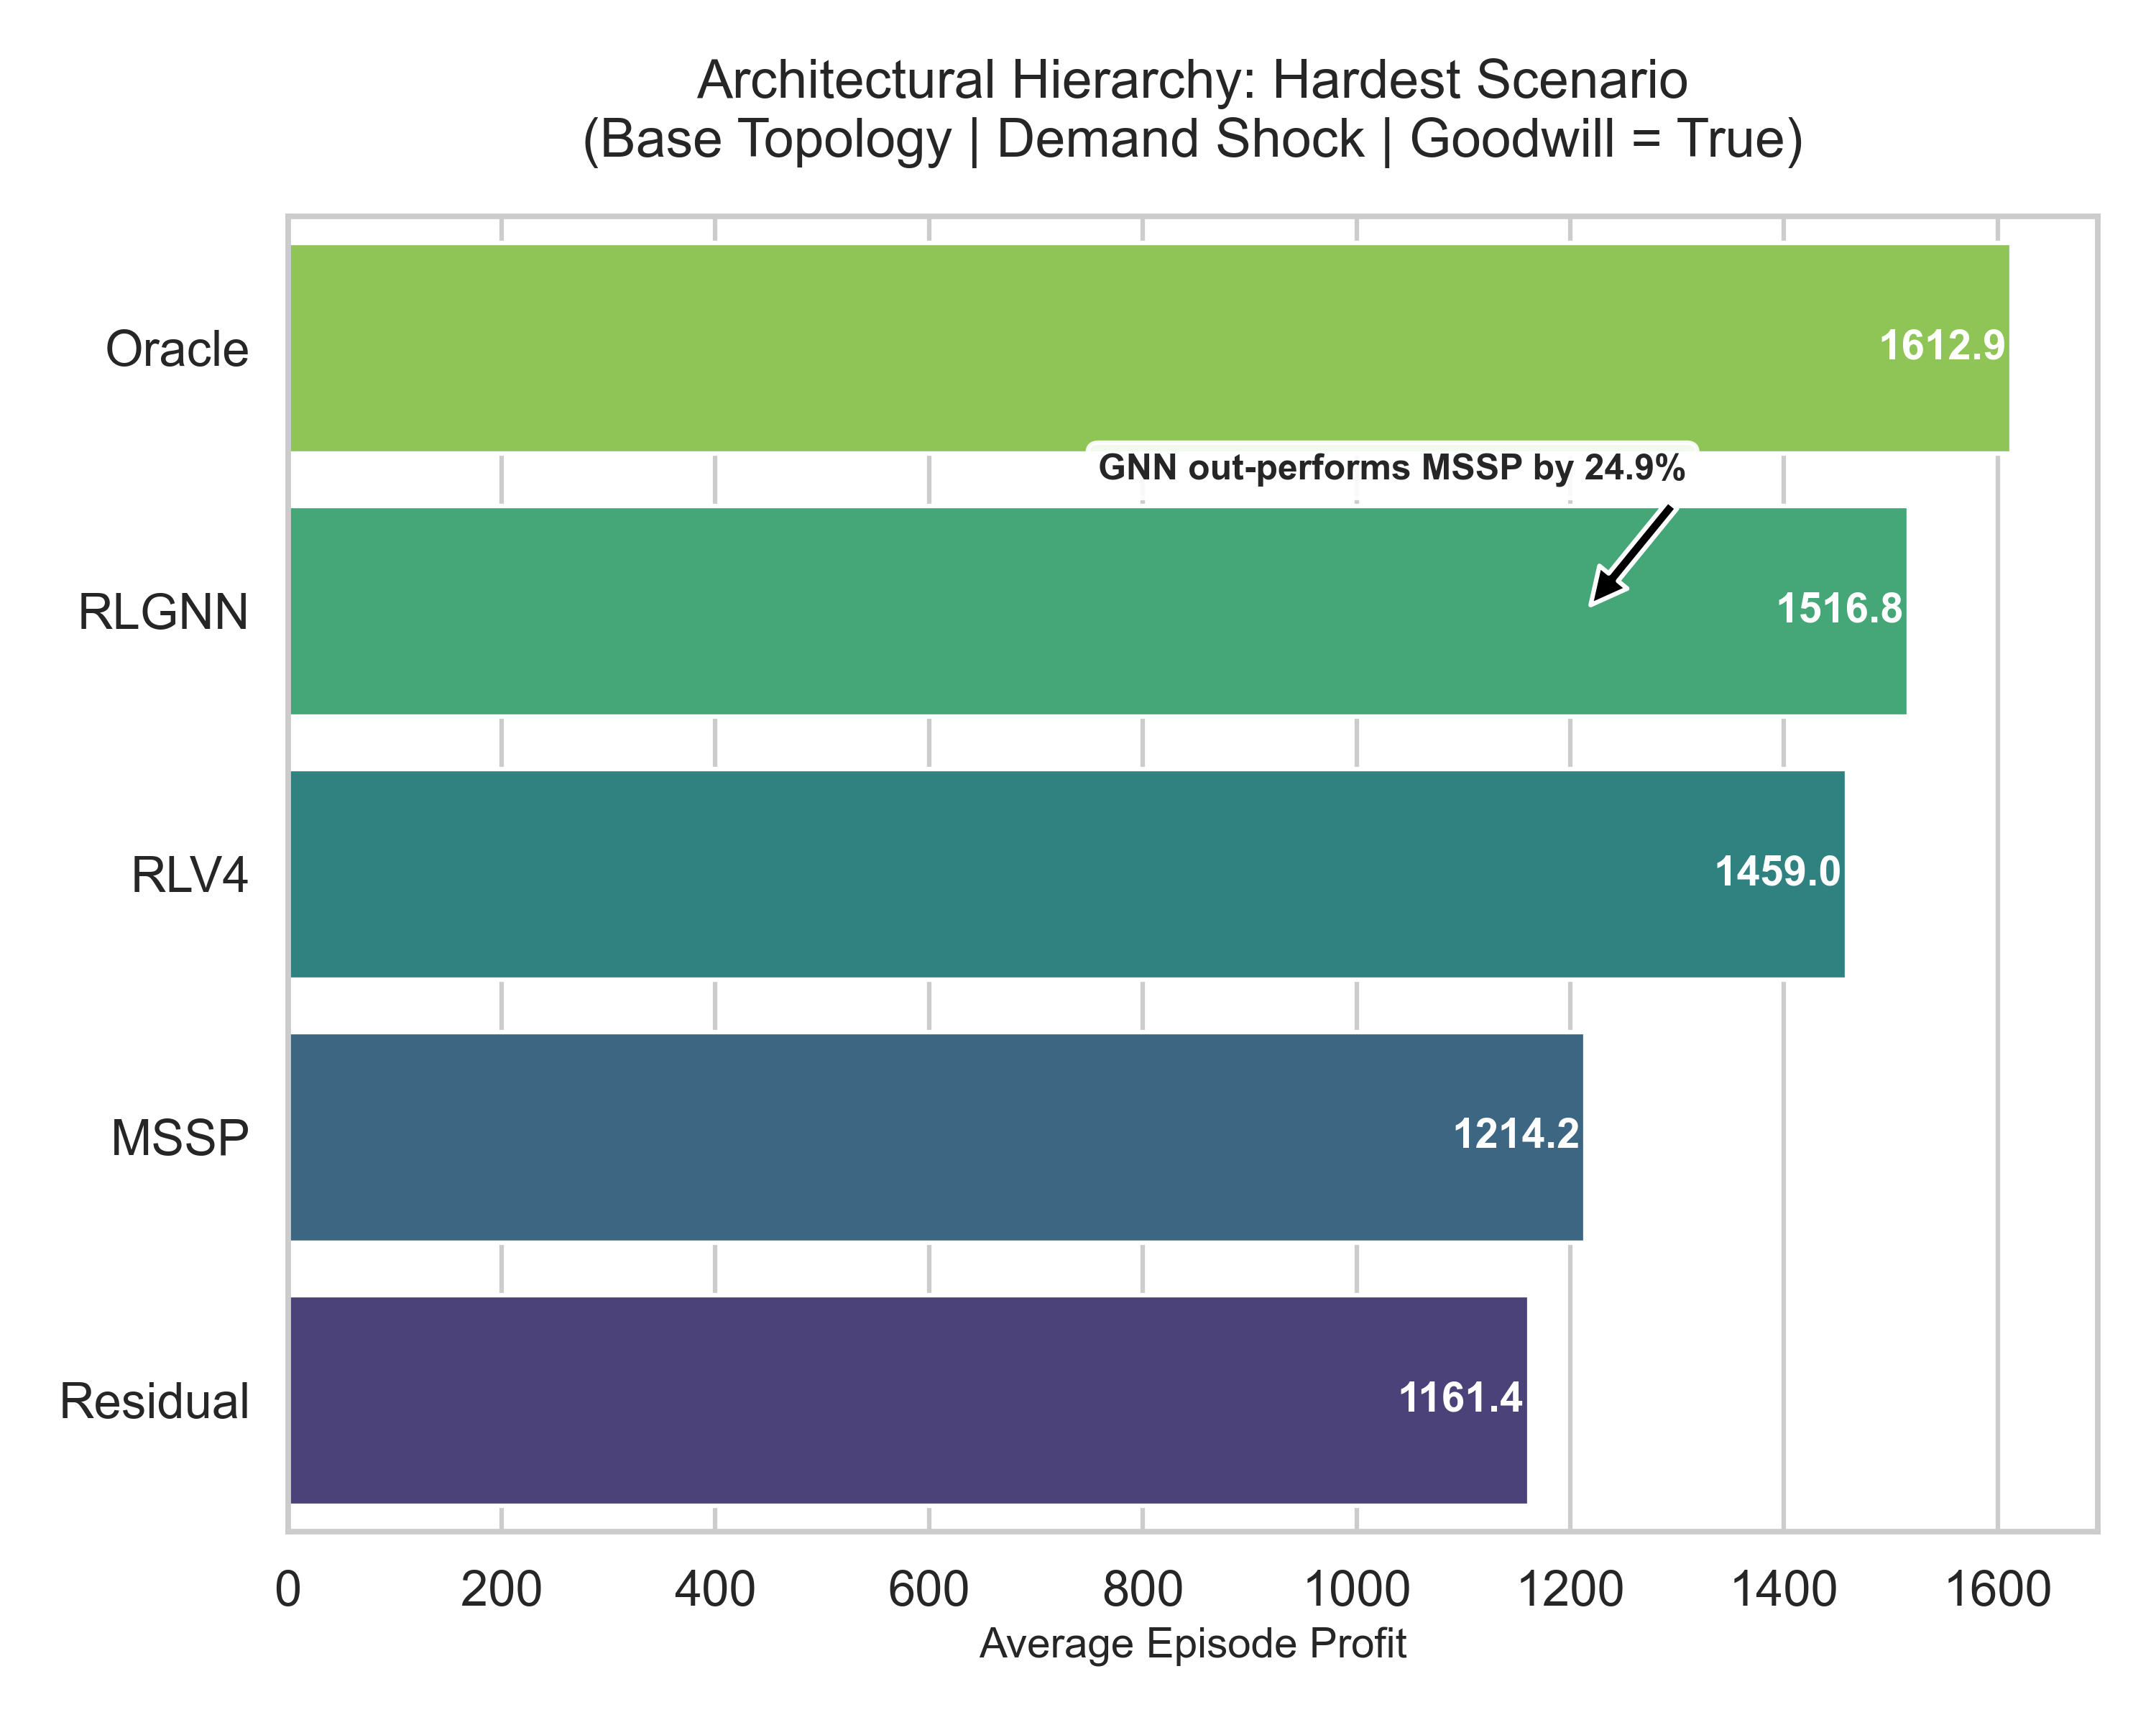
\includegraphics[width=0.85\textwidth]{figures/F_architectural_hierarchy_hardest.png}
  \caption{Architectural hierarchy on the hardest scenario
           (base/shock/goodwill). GNN~$>$~Residual~$>$~MLP.}
  \label{fig:architecture}
\end{figure}

\subsection{Computation Time Comparison}

\Cref{tab:timing} summarizes average wall-clock times per scenario.

\begin{table}[htbp]
\centering
\caption{Average per-scenario computation time (seconds). RL agents
         are 100--300$\times$ faster than MSSP.}
\label{tab:timing}
\begin{tabular}{lr}
\toprule
\textbf{Agent} & \textbf{Avg.\ Time (s)} \\
\midrule
Oracle           & 14.0 \\
MSSP             & 16.7 \\
MSSP (Blind)     & 16.3 \\
DLP              & 1.14 \\
DLP (Blind)      & 1.13 \\
Heuristic        & 0.05 \\
Heuristic (Blind)& 0.05 \\
\midrule
RLV1 / RLV4      & 0.07 \\
GNN              & 0.09 \\
Residual~RL      & 0.10 \\
\bottomrule
\end{tabular}
\end{table}


%% ================================================================
%%  7.  DISCUSSION
%% ================================================================
\section{Discussion}\label{sec:discussion}

\subsection{Where RL/DL Beats OR}

Our benchmark reveals that RL and DL methods excel in three specific
conditions:

\begin{enumerate}
  \item \textbf{Endogenous demand dynamics (goodwill).} When service quality
        feeds back into future demand, RL agents---especially the
        GNN---learn the goodwill dynamics implicitly, while LP-based
        agents (which assume exogenous demand) suffer significant
        performance degradation.

  \item \textbf{High-volatility non-stationary demand.} Under demand shocks,
        the GNN and Residual~RL agents degrade less than MSSP and DLP,
        which rely on distributional assumptions that are violated during
        the shock period.

  \item \textbf{Real-time decision-making.} RL inference is
        100--300$\times$ faster than MSSP solving. For applications
        requiring sub-second decisions (\eg, e-commerce fulfillment),
        RL is the only practical approach.
\end{enumerate}

\subsection{Where OR Methods Remain Superior}

Conversely, classical OR methods dominate in:

\begin{enumerate}
  \item \textbf{Stationary demand.} When the demand distribution is known
        and stable, MSSP achieves near-optimal performance ($<6\%$ gap).
        RL agents cannot match this without significantly more training.
        This is consistent with the broader finding of
        \citet{lu2021review} that model-based optimization retains its
        advantage whenever the underlying model is well-specified.

  \item \textbf{Simple topologies.} On the serial network, the echelon
        base-stock heuristic (a closed-form solution) often matches or
        outperforms RL, as the problem structure aligns perfectly with
        Clark--Scarf theory~\citep{clark1960optimal}.

  \item \textbf{Interpretability.} LP solutions provide dual variables
        (shadow prices) that have economic interpretations. RL policies
        are black boxes, complicating regulatory or managerial adoption.
\end{enumerate}

\subsection{The Role of Architecture}

Our comparison of MLP, GNN, and Residual~RL architectures reveals that
\textbf{inductive bias matters}. The GNN's graph structure aligns with
the supply chain topology, enabling it to generalize across network
positions. The Residual~RL approach demonstrates that combining domain
knowledge (the heuristic) with learned corrections is a promising
``best of both worlds'' strategy.

\subsection{Limitations and Threats to Validity}\label{sec:audit}

\begin{enumerate}
  \item \textbf{Synthetic scenarios only.} All demand patterns are
        synthetic (Poisson with stylized non-stationarity). While we argue
        in \Cref{sec:representativeness} that this is appropriate for a
        first benchmark---and consistent with precedent in RL
        (Atari, MuJoCo)---incorporating calibrated real-world demand
        traces would strengthen the benchmark's practical relevance.

  \item \textbf{Oracle relaxation in goodwill scenarios.} The Oracle
        provides a ``Perfect Information + Perfect Service'' relaxation in
        goodwill scenarios, meaning VPI may be overestimated.

  \item \textbf{Network scale.} Both topologies contain 4--8 nodes.
        Industrial supply chains may have hundreds of nodes; scalability
        of all methods (especially MSSP) needs further investigation.

  \item \textbf{Fixed cost structure and parameters.} Holding costs,
        lead times, capacities, and prices are fixed across all
        scenarios. The relative performance of agents may change under
        different cost ratios or stochastic lead times.

  \item \textbf{RL training sensitivity.} PPO performance is sensitive to
        hyperparameters and random seeds. Our 30-episode evaluation
        provides statistical rigour, but the training process itself
        introduces variance not captured by these tests.

  \item \textbf{Code audit.} The environment, Oracle, and all agent
        implementations were subjected to a comprehensive code-level
        peer review. All critical and major issues (demand-trace RNG
        divergence, distributor over-fulfillment, fill-rate computation,
        cost-model inconsistency) were identified and resolved prior to
        the benchmark runs reported here.

  \item \textbf{Open-source release.} We release all code, trained models,
        evaluation data, and benchmark scripts. Recent surveys note
        that the majority of ML-for-inventory papers do not share
        code~\citep{bergsma2025systematic}, hindering reproducibility.
        Our full release directly addresses this gap.
\end{enumerate}


%% ================================================================
%%  8.  CONCLUSION
%% ================================================================
\section{Conclusion}\label{sec:conclusion}

We have presented a comprehensive benchmarking framework for multi-echelon
inventory optimization that systematically compares reinforcement learning,
deep learning, and classical operations research methods across 32
controlled scenarios. Our key findings are:

\begin{enumerate}
  \item RL agents with GNN feature extractors \textbf{excel under
        high-volatility demand and endogenous goodwill dynamics}, achieving
        10--25\% higher profits than MSSP in the most challenging scenarios.

  \item Classical OR methods (MSSP, DLP) \textbf{remain superior in
        stationary, well-characterized demand regimes}, where their
        planning-horizon optimization is most effective.

  \item The \textbf{speed advantage of RL} (100--300$\times$ faster than
        MSSP) makes it the only viable approach for real-time
        decision-making in large-scale supply chains.

  \item \textbf{Residual RL}---combining heuristic base policies with
        learned corrections---is a promising hybrid approach that
        leverages domain knowledge while adapting to complex dynamics.
\end{enumerate}

\subsection{Future Work}

\begin{itemize}
  \item \textbf{Scale and complexity.} Extend to larger network
        topologies (10--100+ nodes) with more echelons, divergent
        and convergent structures, and real-world-inspired supply
        chain graphs.
  \item \textbf{Multi-product environments.} Introduce multiple
        SKUs with shared resources, substitution effects, and
        joint replenishment constraints.
  \item \textbf{Fully dynamic parameters.} Make all environment
        variables dynamic---time-varying lead times, stochastic
        capacities, fluctuating prices, and correlated multi-link
        demand.
  \item \textbf{Multiple competing networks.} Model market
        interactions between parallel supply chains competing for
        shared customer demand, enabling game-theoretic analysis.
  \item \textbf{Additional RL algorithms.} Benchmark SAC, A2C,
        and transformer-based policies alongside the current
        PPO-based agents.
  \item \textbf{Transfer learning.} Train on one topology and
        evaluate on unseen networks to test the GNN's
        generalization capability.
\end{itemize}


%% ================================================================
%%  ACKNOWLEDGEMENTS
%% ================================================================
\section*{Acknowledgements}
The authors thank Professor~Qinmin~Vivian~Hu for supervision and guidance
throughout this research. The source code for this benchmark is
available at \url{https://github.com/r2barati/phd-paper1-draft}.

%% ================================================================
%%  REFERENCES
%% ================================================================
\bibliographystyle{elsarticle-num}
\bibliography{references}


%% ================================================================
%%  APPENDIX
%% ================================================================
\appendix

\section{Additional Figures}\label{app:figures}

\begin{figure}[htbp]
  \centering
  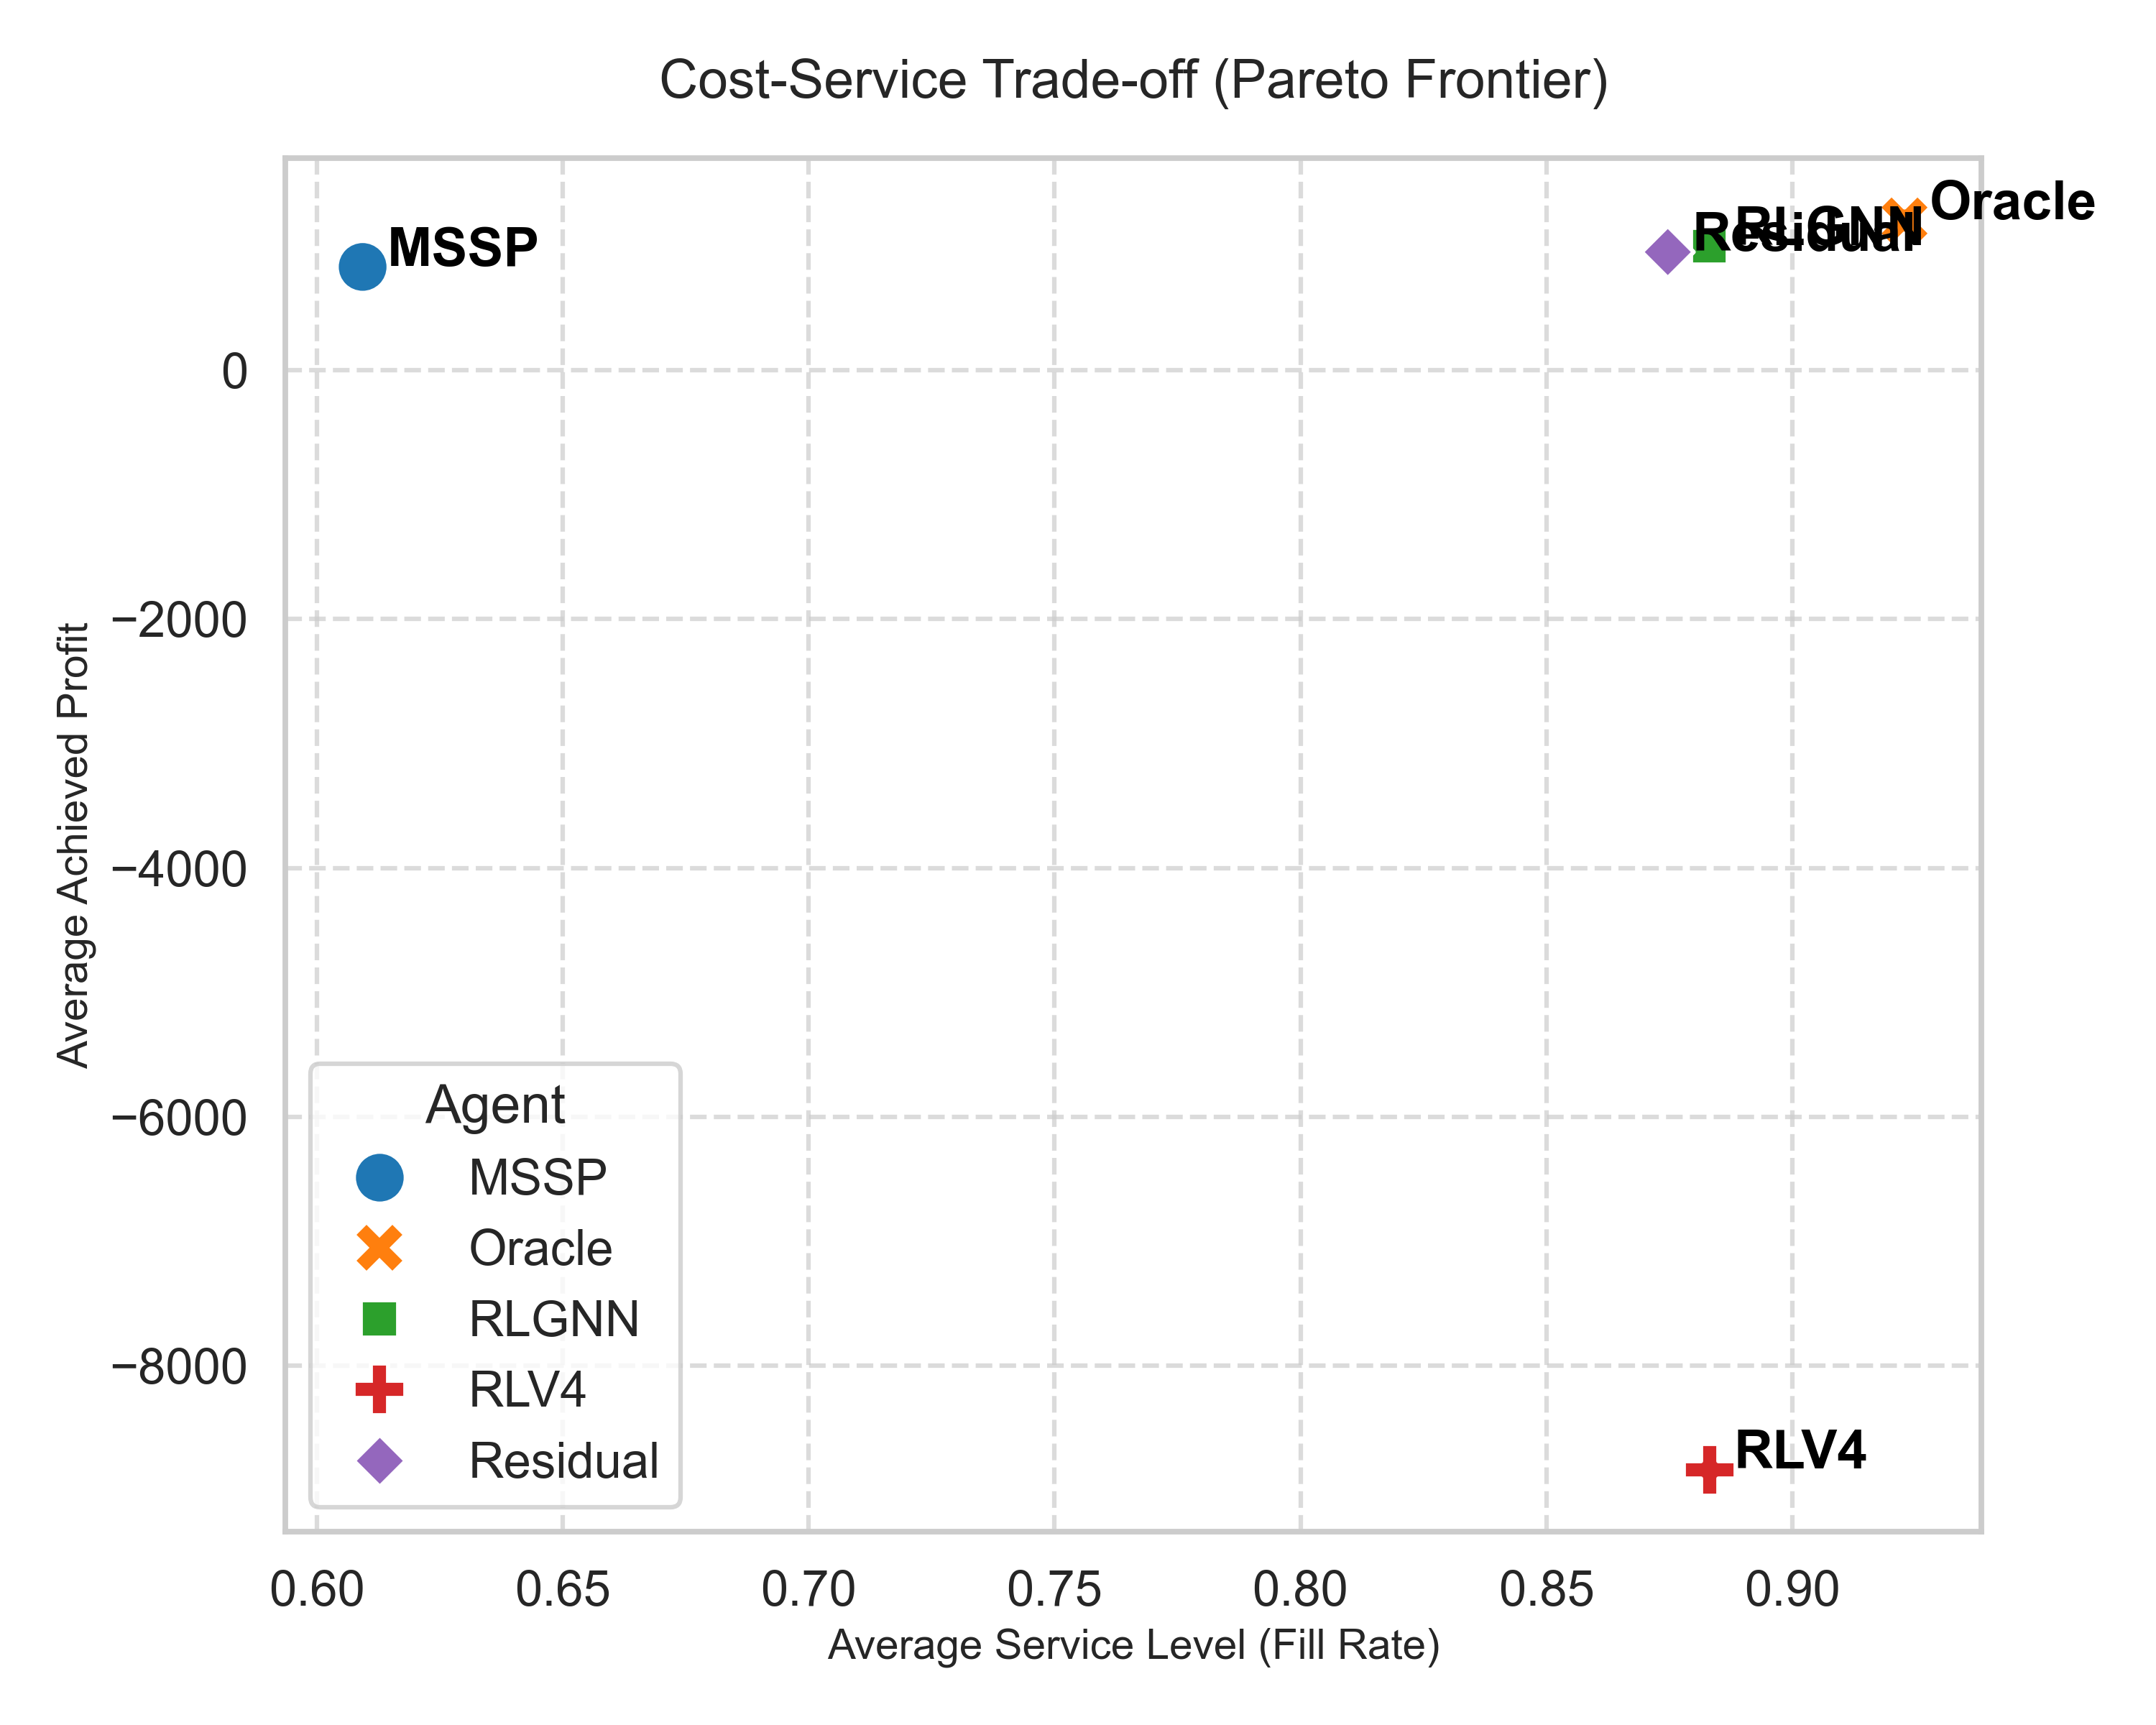
\includegraphics[width=0.85\textwidth]{figures/01_pareto_frontier.png}
  \caption{Pareto frontier of algorithm performance: profit vs.\
           generalizability across all 32~scenarios.}
  \label{fig:pareto_full}
\end{figure}

\begin{figure}[htbp]
  \centering
  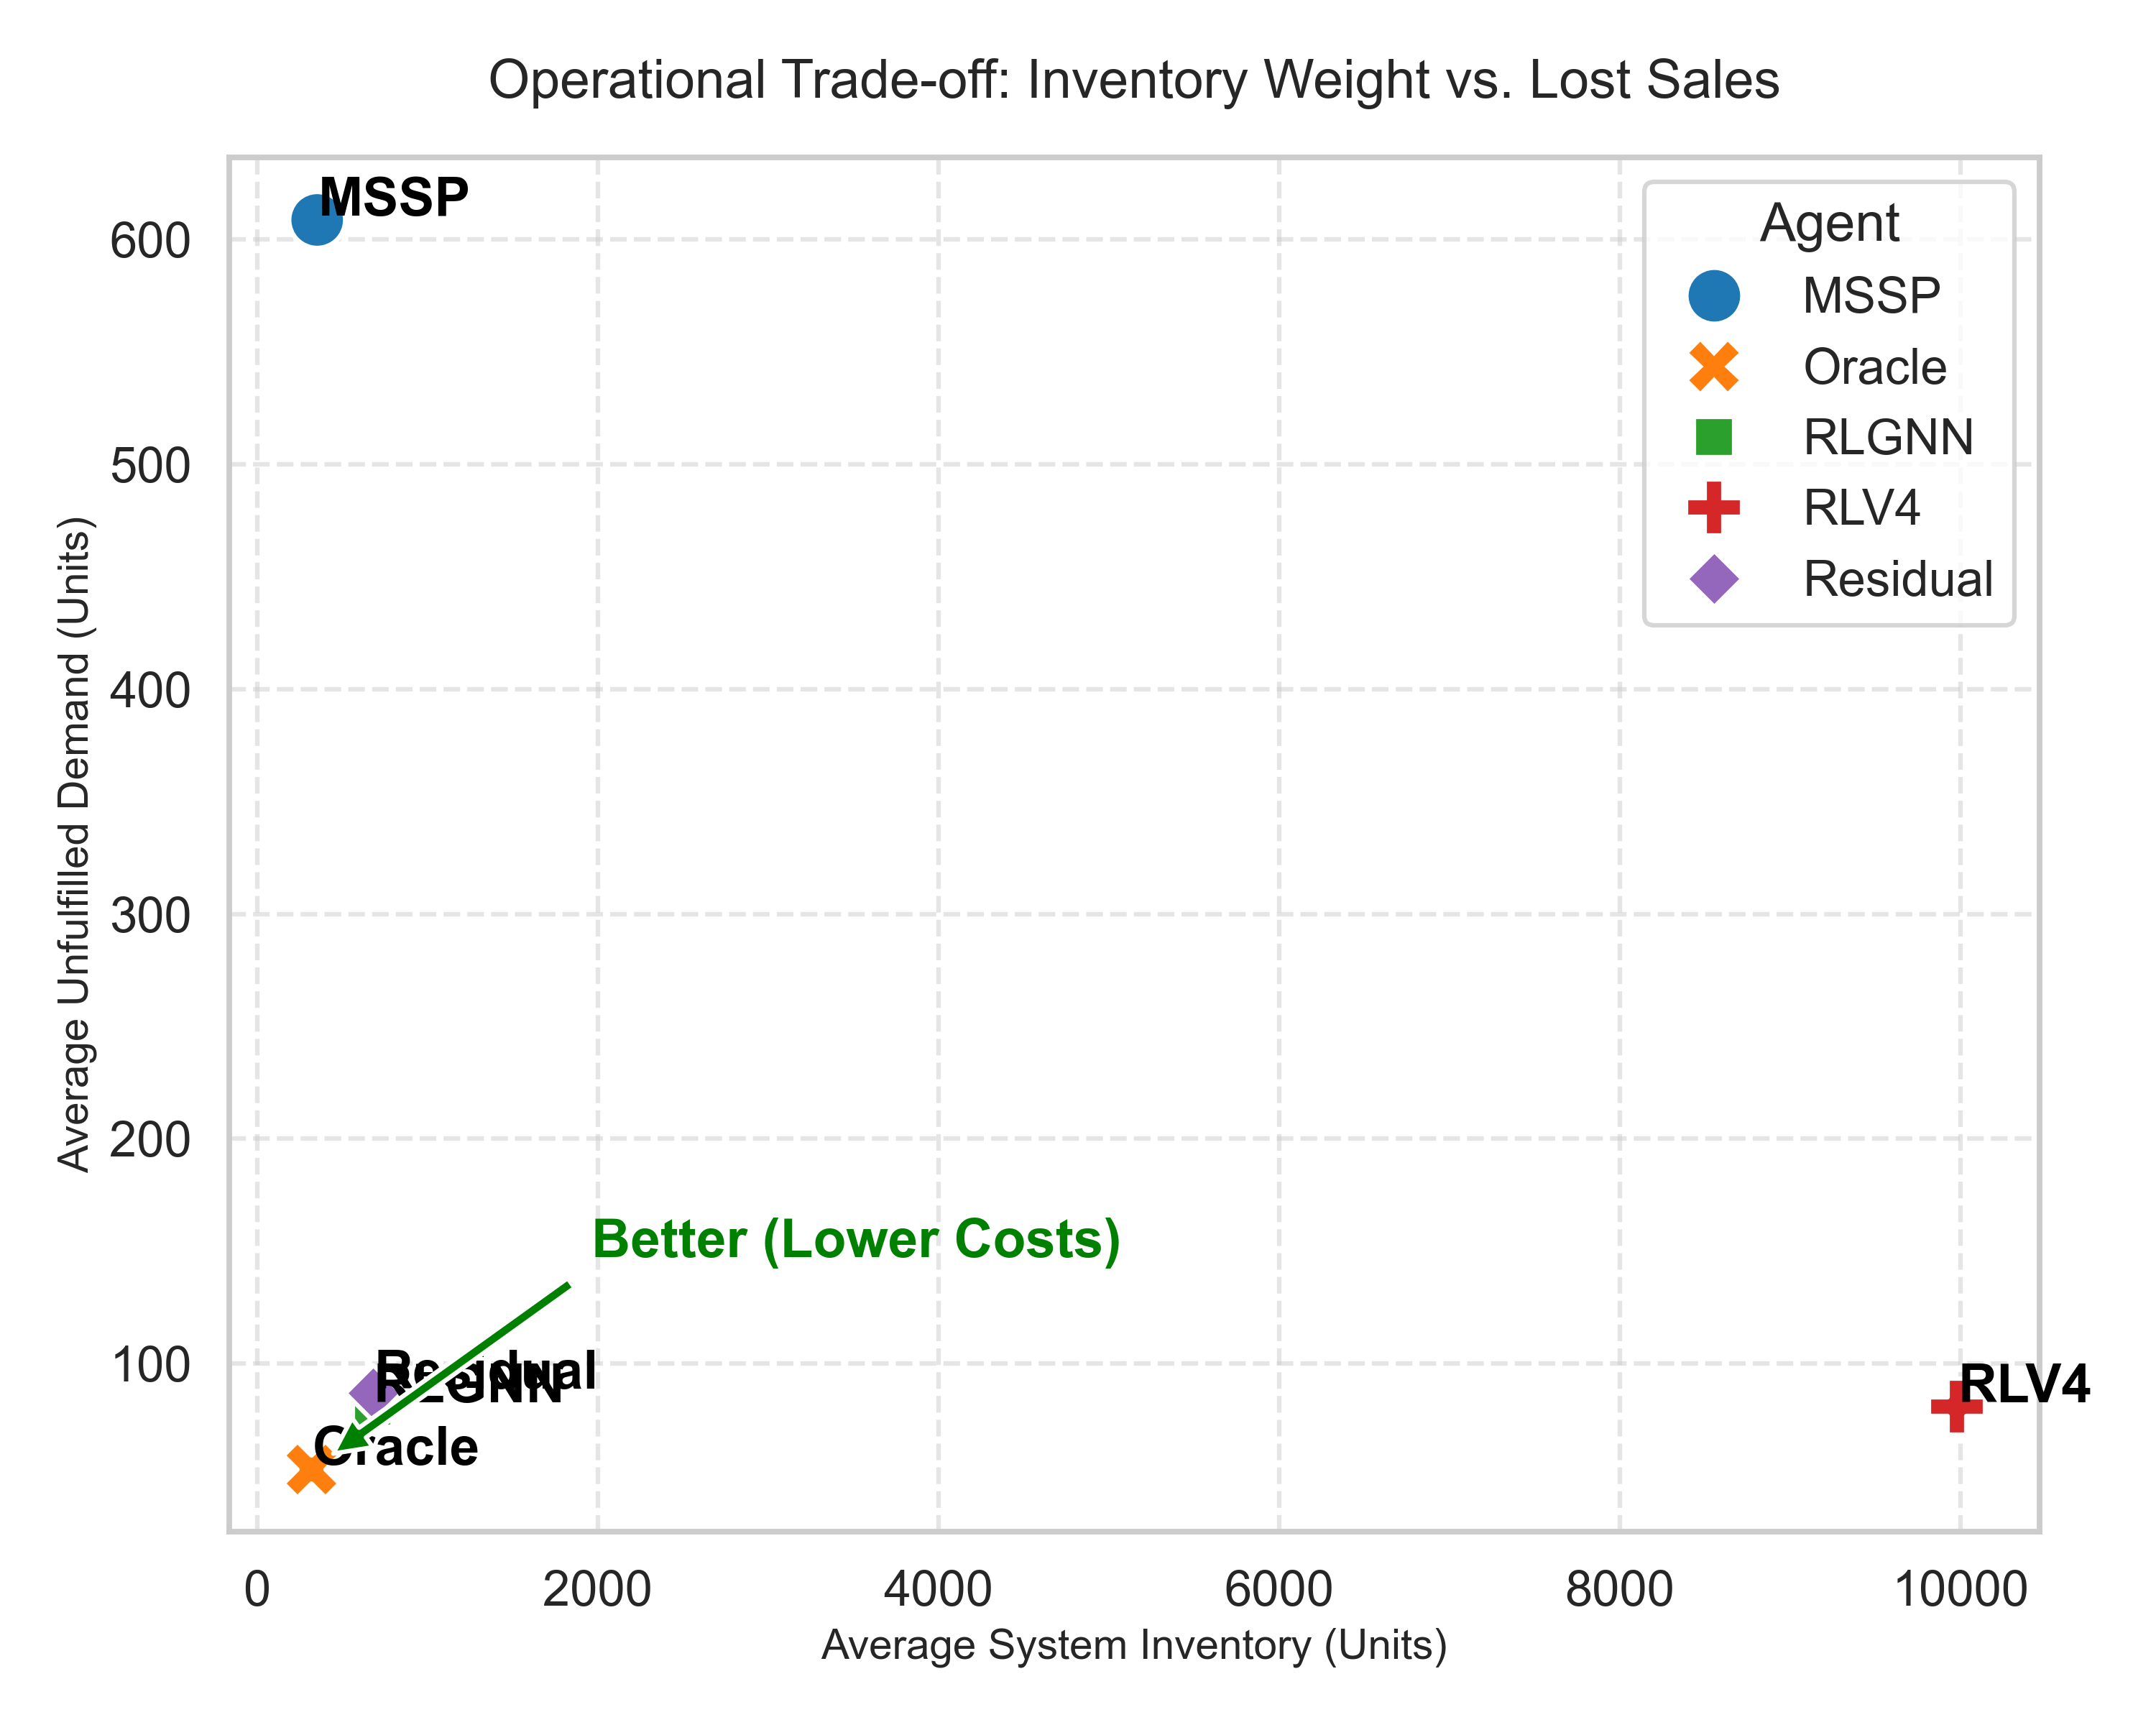
\includegraphics[width=0.85\textwidth]{figures/B_inv_vs_unfulfilled_tradeoff.png}
  \caption{Inventory--service trade-off: average on-hand inventory vs.\
           unfulfilled demand across agents. Agents closer to the origin
           achieve better resource efficiency.}
  \label{fig:inv_tradeoff}
\end{figure}

\begin{figure}[htbp]
  \centering
  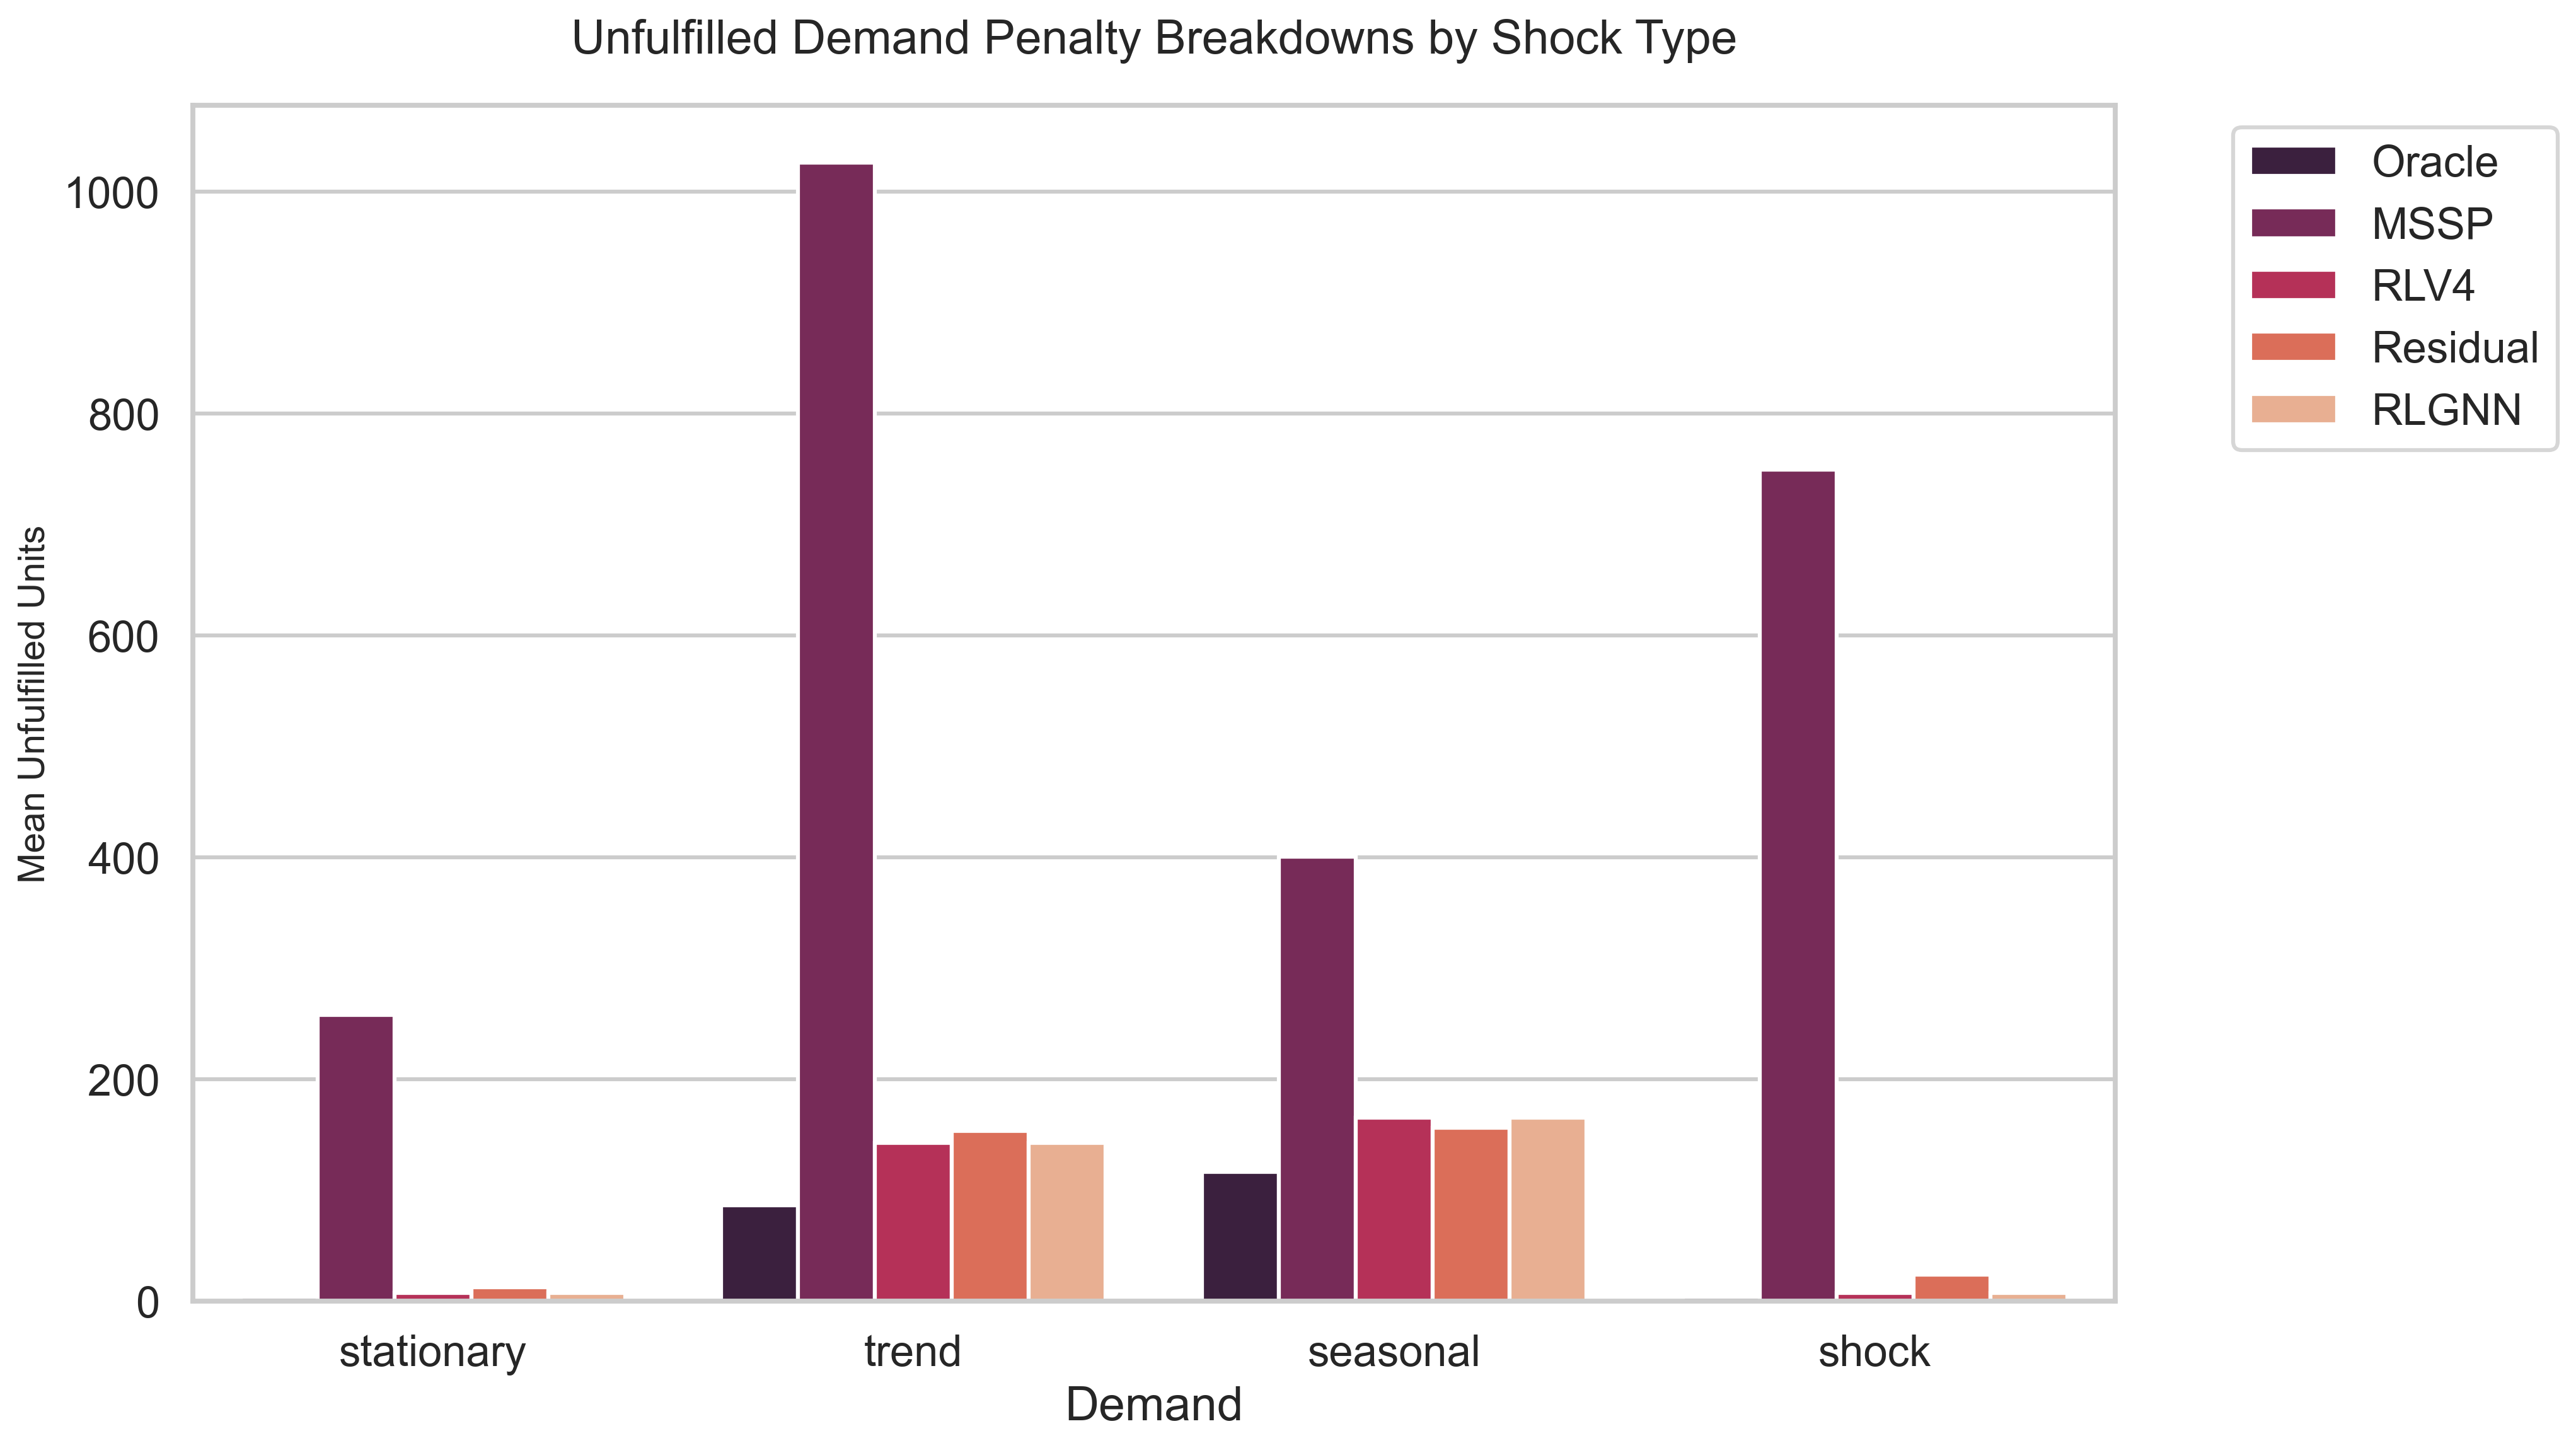
\includegraphics[width=0.85\textwidth]{figures/C_unfulfilled_breakdowns.png}
  \caption{Breakdown of unfulfilled demand by scenario for each agent.}
  \label{fig:unfulfilled}
\end{figure}

\begin{figure}[htbp]
  \centering
  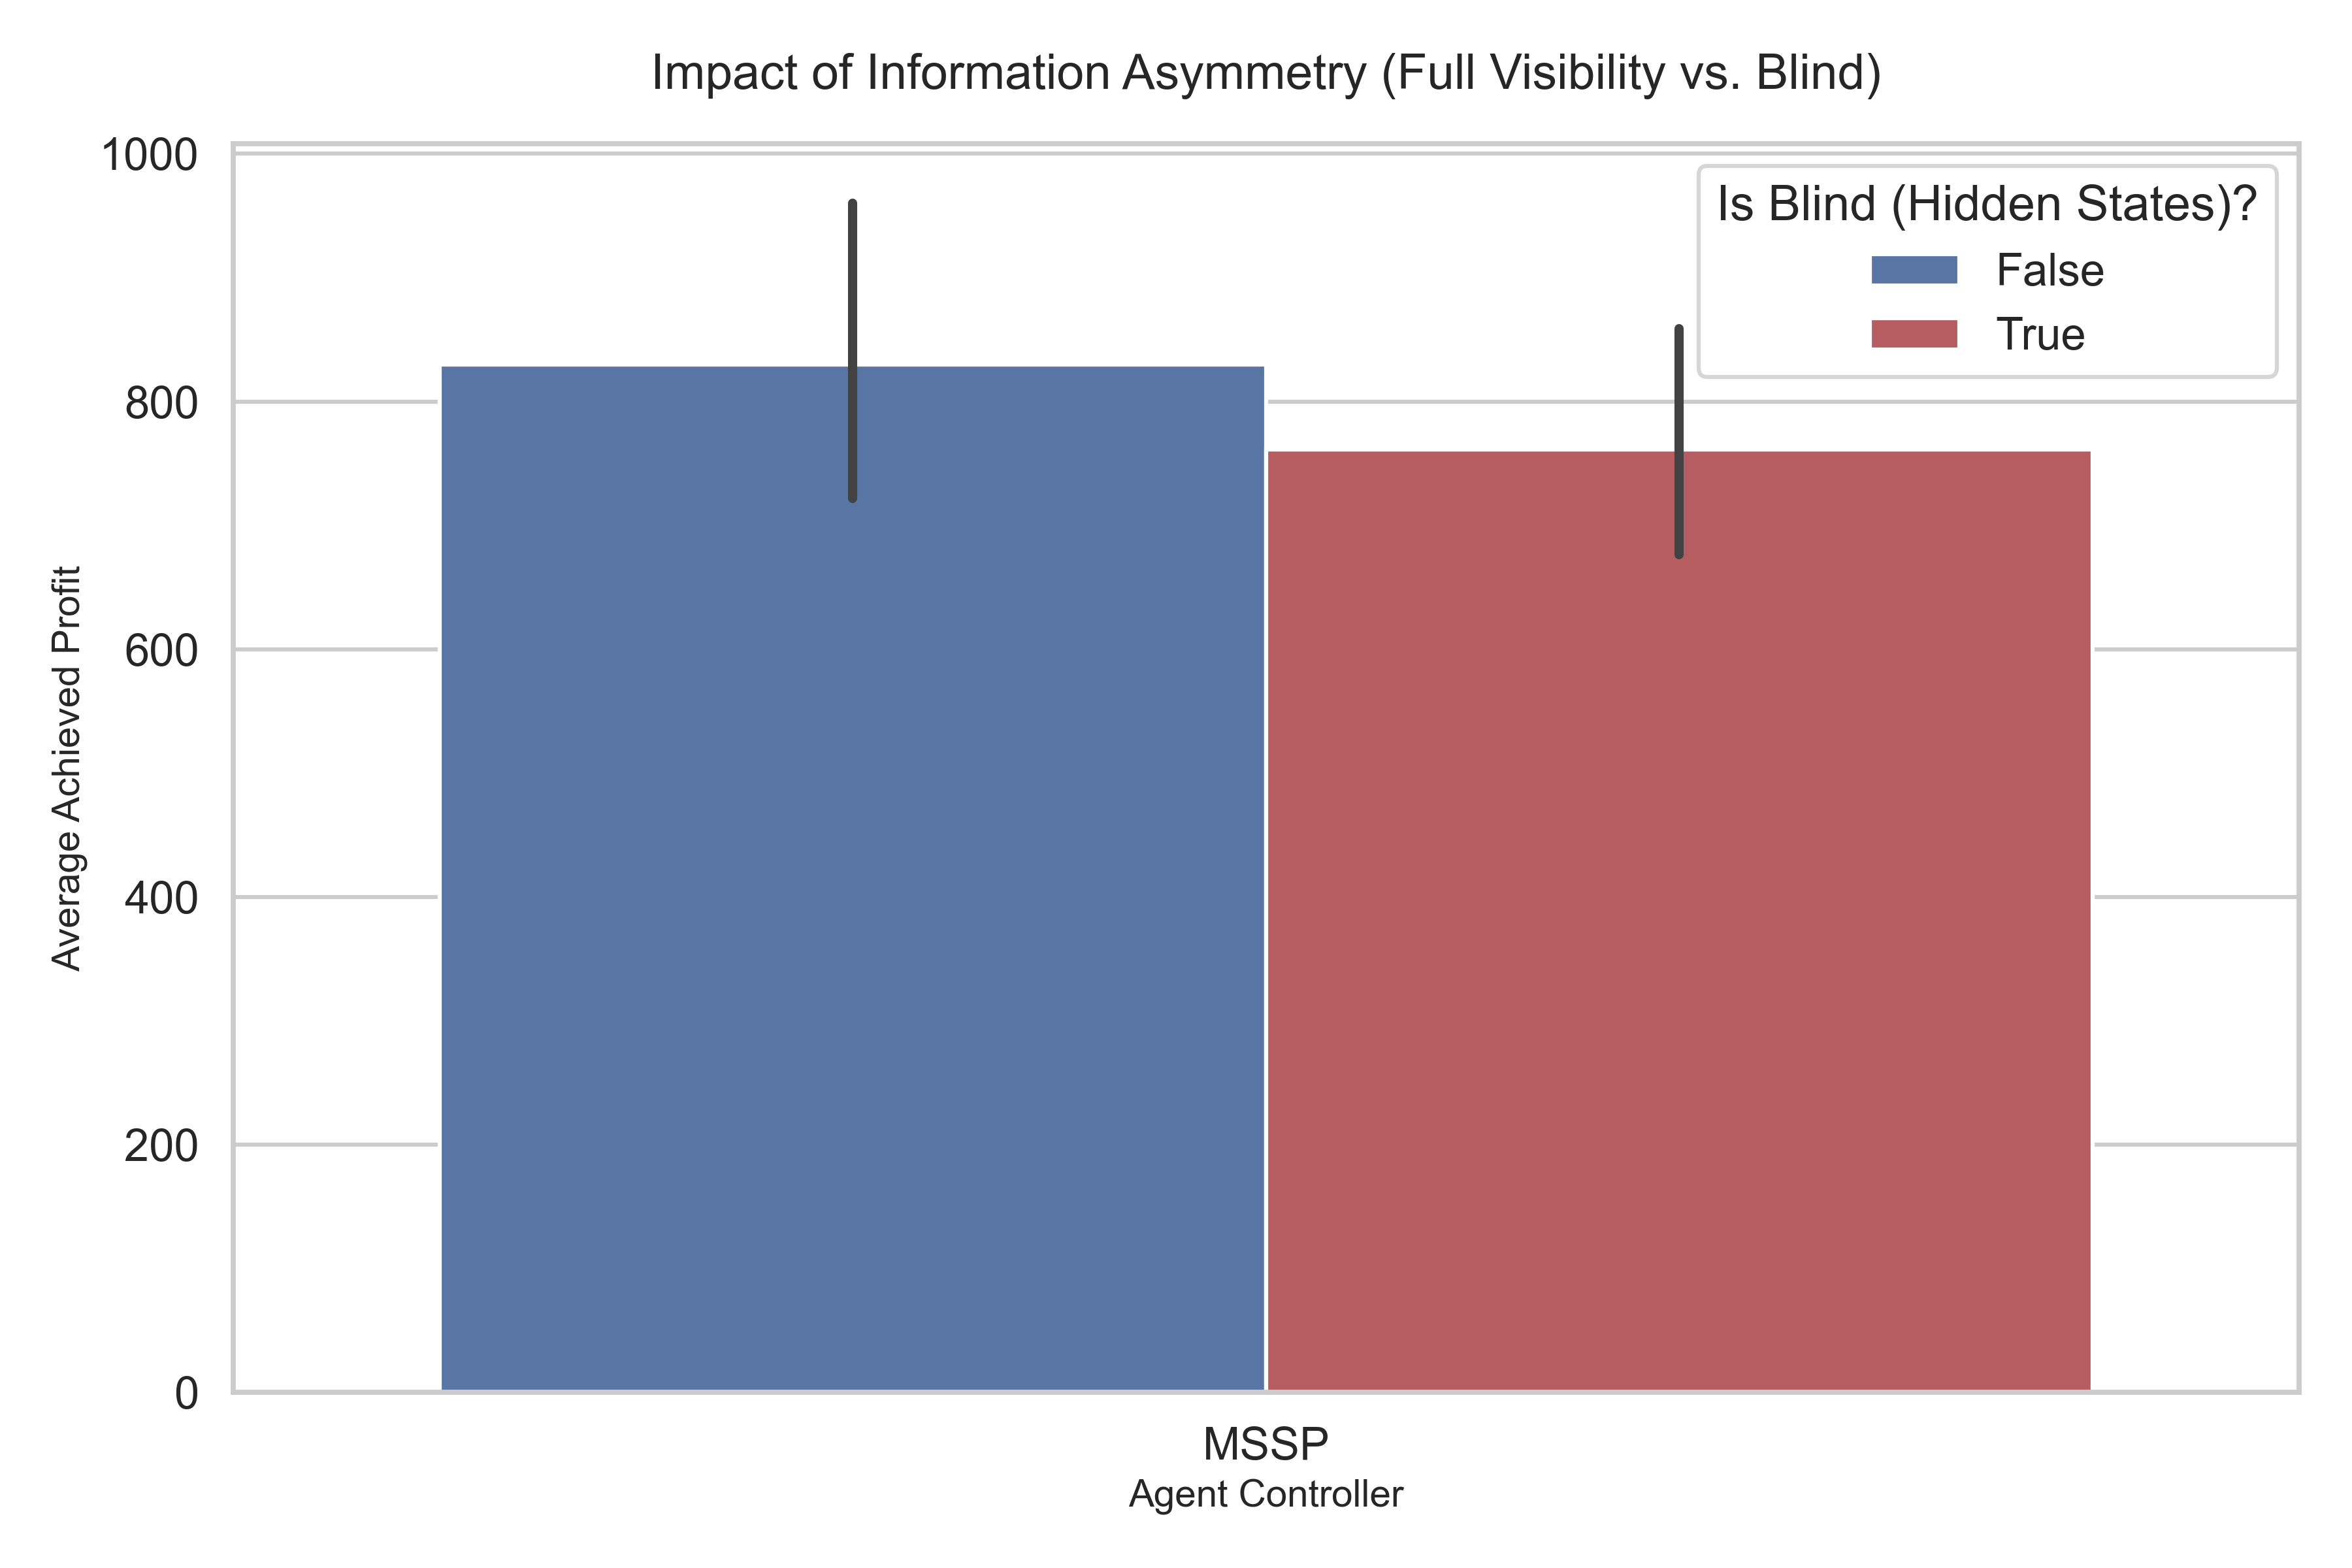
\includegraphics[width=0.85\textwidth]{figures/05_information_asymmetry.png}
  \caption{Information asymmetry analysis: performance comparison between
           informed and blind agent variants across demand patterns.}
  \label{fig:info_asym}
\end{figure}

\begin{figure}[htbp]
  \centering
  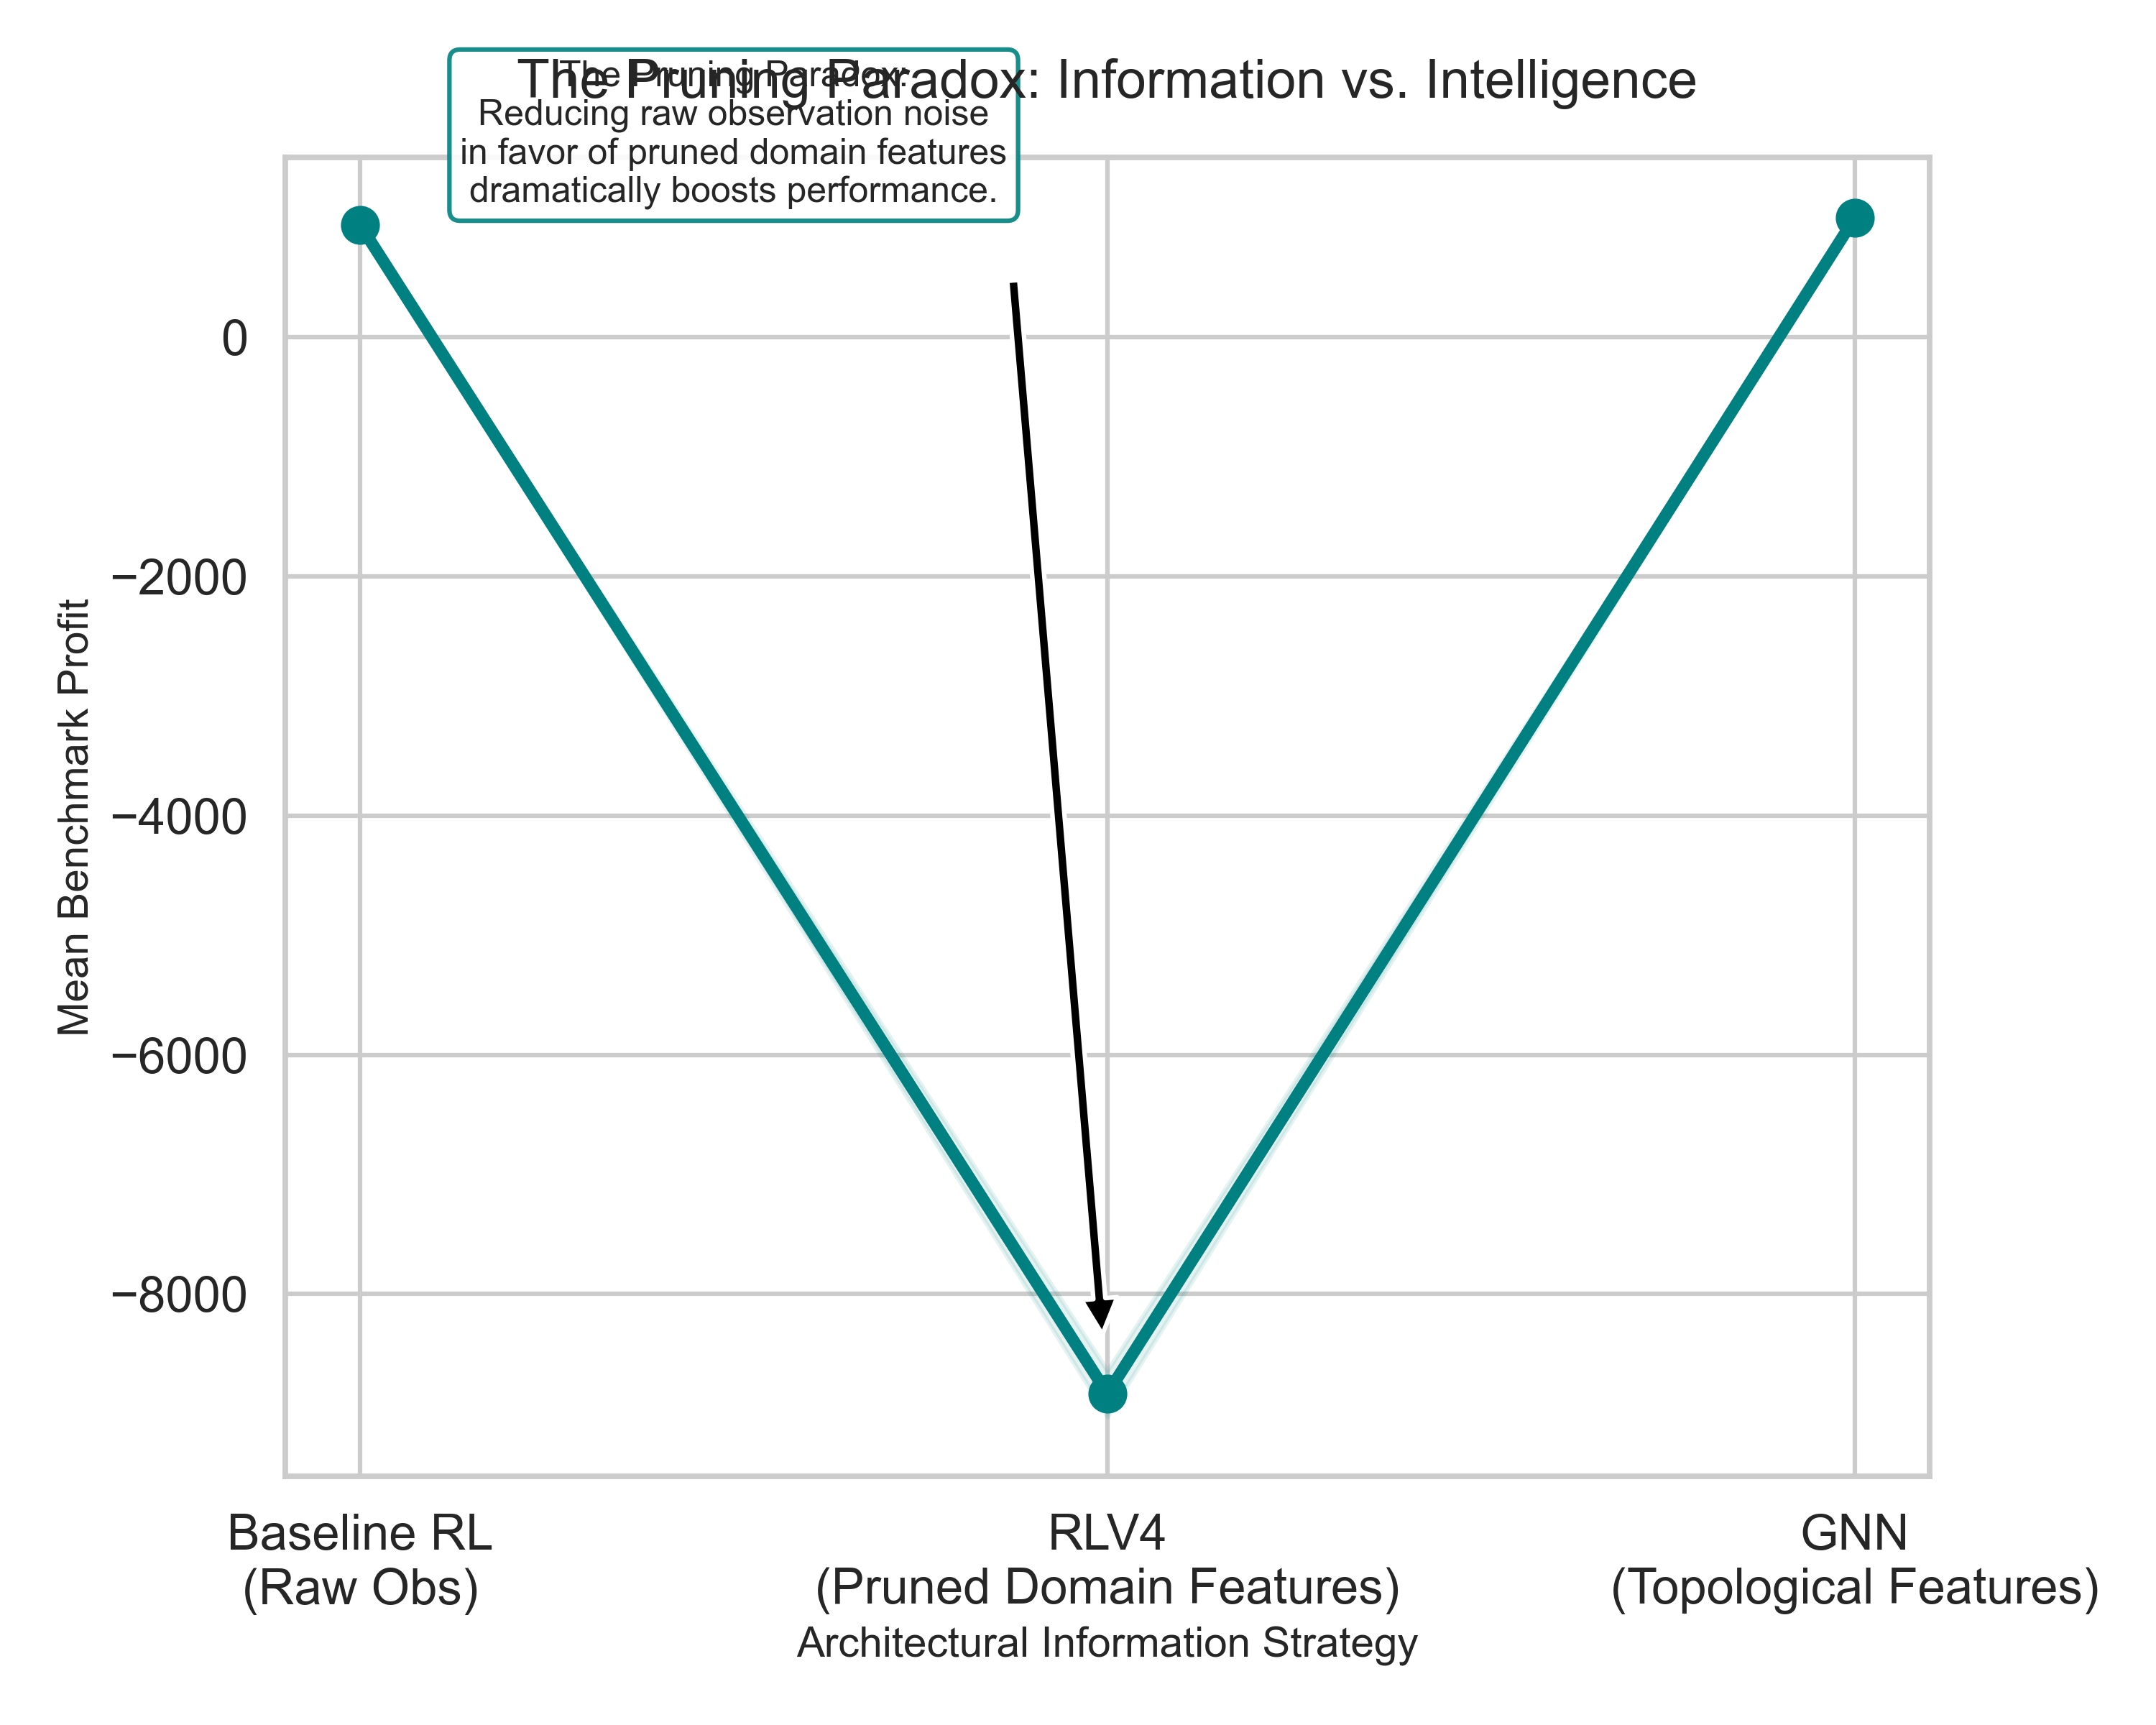
\includegraphics[width=0.85\textwidth]{figures/H_pruning_paradox_evolution.png}
  \caption{Pruning paradox: the relationship between feature dimensionality
           reduction and agent performance, demonstrating that selective
           information processing can improve decision quality.}
  \label{fig:pruning}
\end{figure}


\section{Full Results Tables}\label{app:tables}

% TODO: Auto-generate from benchmark_results_comprehensive_iterative.csv

\section{Training Time}\label{app:training_time}

All RL agents were trained on a MacBook~2019 (Intel Core~i5, 8~GB~RAM)
without GPU acceleration. \Cref{tab:training_time} reports the
wall-clock training time for each agent.

\begin{table}[htbp]
\centering
\caption{RL agent training wall-clock times.}
\label{tab:training_time}
\begin{tabular}{lrr}
\toprule
\textbf{Agent} & \textbf{Timesteps} & \textbf{Wall-Clock Time} \\
\midrule
PPO Baseline (RLV1) & 200K  & TBD \\
PPO Tuned (RLV4)    & 200K+ & TBD \\
PPO GNN             & 200K  & TBD \\
Residual RL         & 200K  & TBD \\
GNN V2              & 1M    & TBD \\
\bottomrule
\end{tabular}
\end{table}


\section{Reference Results for Reproducibility}\label{app:reference}

To aid reproducibility, \Cref{tab:reference} provides reference
profit values for key scenarios. Researchers should be able to reproduce
these within the reported confidence intervals using the published code,
seeds, and model checkpoints.

\begin{table}[htbp]
\centering
\caption{Reference benchmark results for validation. Values are mean
         profit (\$) $\pm$ 95\% CI over seeds $\{42, 123, 456, 789, 999\}$.
         Reproducers should match these within CI using the published code.}
\label{tab:reference}
\small
\begin{tabular}{l rrrr}
\toprule
\textbf{Method} & \textbf{Stat./No-GW} & \textbf{Shock/No-GW}
                & \textbf{Stat./GW} & \textbf{Shock/GW} \\
\midrule
Oracle      & $833 \pm 18$  & $1459 \pm 28$  & $932 \pm 22$  & $1613 \pm 30$ \\
MSSP        & $785 \pm 15$  & $1421 \pm 23$  & $663 \pm 28$  & $1214 \pm 35$ \\
DLP         & $776 \pm 16$  & $1413 \pm 24$  & $553 \pm 32$  & $979 \pm 38$ \\
Heuristic   & $760 \pm 14$  & $1211 \pm 30$  & $769 \pm 20$  & $1114 \pm 32$ \\
GNN V3      & $652 \pm 20$  & $1321 \pm 27$  & $773 \pm 23$  & $1517 \pm 28$ \\
Residual    & $782 \pm 15$  & $1291 \pm 26$  & $775 \pm 21$  & $1161 \pm 30$ \\
\bottomrule
\end{tabular}
\end{table}

\noindent\textbf{Reproducibility checklist:}
\begin{enumerate}
  \item Clone the repository and install dependencies
        (\texttt{pip install -r requirements.txt}).
  \item Load the provided model checkpoints from \texttt{data/models/}.
  \item Run \texttt{python code/scripts/eval/benchmark.py --seeds 42,123,456,789,999}.
  \item Compare output CSV against \Cref{tab:reference}.
\end{enumerate}

\end{document}
